\documentclass[10pt]{article}  

%%%%%%%% PREAMBOLO %%%%%%%%%%%%
\usepackage[english]{babel}
\usepackage[utf8]{inputenc}
\usepackage{amssymb}
\usepackage{graphicx}
\usepackage{color}
\usepackage{subfigure}
\usepackage{ulem}
\usepackage{biblatex}
\usepackage[most]{tcolorbox}
\addbibresource{bib/citations.bibtex}
%%%%%%%%%%%%%CODE%%%%%%%%%%%%%%%%%%%%%%
\usepackage{listings}
\usepackage{caption}
\DeclareCaptionFont{white}{\color{white}}
\DeclareCaptionFormat{listing}{%
  \parbox{\textwidth}{\colorbox{gray}{\parbox{\textwidth}{#1#2#3}}\vskip-4pt}}
\captionsetup[lstlisting]{format=listing,labelfont=white,textfont=white}
\lstset{frame=lrb,xleftmargin=\fboxsep,xrightmargin=-\fboxsep}
%%%%%%%%%%%%%CODE%%%%%%%%%%%%%%%%%%%%%%
\usepackage{float}
\usepackage{array}
\usepackage{capt-of}
\usepackage{enumerate}
\usepackage{sidecap}
\sidecaptionvpos{figure}{c}
\usepackage{caption}
\usepackage{commath}
 
\usepackage{anysize}
\marginsize{2cm}{2cm}{2cm}{2cm}


% TABLES
\usepackage{array}
\newcolumntype{P}[1]{>{\centering\arraybackslash}p{#1}}
\newcolumntype{M}[1]{>{\centering\arraybackslash}m{#1}}
\usepackage{makecell}



% COLORED TABLES
\usepackage{tcolorbox}
\tcbuselibrary{listingsutf8}
\newtcolorbox[auto counter, number within=section]{example}[2][]
{colback=black!5!white,colframe=black!75!black,
fonttitle=\bfseries, title=Note}

\newtcolorbox[auto counter, number within=section]{Warning}[2][]
{colback=red!5!white,colframe=red!75!black,
fonttitle=\bfseries, title=Very Important}

\usepackage[colorlinks=true,plainpages=false,citecolor=blue,linkcolor=blue]{hyperref}
\usepackage{fancyhdr} 
\pagestyle{fancy}
\fancyhf{}
\fancyhead[L]{\footnotesize Computer Architectures and Operating Systems project}
\fancyfoot[C]{\thepage} 
\renewcommand{\footrulewidth}{0.4pt}


\usepackage{listings} 
\definecolor{dkgreen}{rgb}{0,0.6,0} 
\definecolor{gray}{rgb}{0.5,0.5,0.5} 
% CODICE BASH
\lstset{language=bash, keywords={enable, target, kernel, machine, monitor, cd, sudo, apt, install, make, git, which}}
\definecolor{codegreen}{rgb}{0,0.6,0}
\definecolor{codegray}{rgb}{0.5,0.5,0.5}
\definecolor{codepurple}{rgb}{0.58,0,0.82}
\definecolor{backcolour}{rgb}{0.95,0.95,0.92}

\lstdefinestyle{mystyle}{
    backgroundcolor=\color{backcolour},   
    commentstyle=\color{codegreen},
    keywordstyle=\color{magenta},
    numberstyle=\tiny\color{codegray},
    stringstyle=\color{codepurple},
    basicstyle=\ttfamily\footnotesize,
    breakatwhitespace=false,         
    breaklines=true,                 
    captionpos=b,                    
    keepspaces=true,                                  
    numbersep=5pt,                  
    showspaces=false,                
    showstringspaces=false,
    showtabs=false,                  
    tabsize=2
}

\lstset{style=mystyle}

%%%%%%%% END PREAMBOLO %%%%%%%%%%%%

\begin{document}
\begin{center}																	
\newcommand{\HRule}{\rule{\linewidth}{0.5mm}}									
\textsc{\Large Project Assignment}\\[0.5cm]
\vspace*{1cm}																	
\HRule \\[0.4cm]																
{ \huge \bfseries Computer Architectures and Operating Systems }\\[0.4cm]
\HRule \\[5.5cm]																	
 																				
																					
\begin{minipage}{0.4\textwidth}													
\begin{flushleft} \large															
\textit{Authors:}\\
A. A. Antonini\\
F. Goffredo\\
G. Pizzenti \\
F. Rollo \\
Group 24\\
\end{flushleft}																		
\end{minipage}		
																
\begin{minipage}{0.5\textwidth}		
\vspace{-4.5cm}											
\begin{flushright} \large															
\textit{Professor:} \\
Stefano Di Carlo																						
\end{flushright}																	
\end{minipage}	
\vspace*{1cm}

\vspace{2cm} 																				
\begin{center}																					
{\large A.A. 2023-24}																	
 			\end{center}												  						
\end{center}							 											
												 											
																					
\newpage																		
%%%%%%%%%%%%%%%%%%%% END INTRODUCTION %%%%%%%%%%%%%%%%%%%%%%%%%%%%%%%%

\tableofcontents 

\newpage
\part{Setup Tutorial and first steps}
\section{Introduction}
\subsection{What are QEMU and Emulation?}
This tutorial explains how to set up a \textit{QEMU} to emulate a popular development board, the mps2 using an an385 FPGA (as described in the ARM AN385 Application Note). Then, we will run a Real Time OS (FreeRTOS) on the emulated environment.
\\
\vspace*{0.2cm}
In our case, an \textbf{emulator} is a \textbf{software} that makes an host system, our PC, behave like another, namely, a development board with an ARM Cortex-M3 processor on board. This is achieved in QEMU in (Full) System Emulation mode, which is used to build a virtualized version of the FPGA, on top of which we can run any OS developed for our chosen CPU.
\\
\vspace*{0.2cm}
As we can see from the FreeRTOS configuration file, the OS’ internal clock is declared as 25MHz (we set it the same as the MPS2’s SYSTICK), while the FreeRTOS Tick, generated from the internal clock, will produce interrupts at 0.02 MHz.

\section{Installing QEMU and running the FreeRTOS demo}
Now that we have laid the bases of Real Time operations, it’s time to install the QEMU emulator on our system and say our Hello to the World (in our case it will be more of a friendly blink of a led, in perfect hardware-testing tradition).
\subsection{Installing QEMU}
\begin{example}{Note}
The following commands have been tested on Ubuntu Linux 22.10.
\end{example}

First of all, let's install QEMU on our system:
\begin{lstlisting}
sudo apt install qemu-system
\end{lstlisting}
Then, let's download and unzip the FreeRTOS Kernel and the demo project bundled with it:
\begin{lstlisting}
git clone https://github.com/FreeRTOS/FreeRTOS.git --recurse-submodules
\end{lstlisting}

\begin{example}{Note}
    A lot of files in this folder are not needed for our purposes. Feel free to delete any subfolder dedicated to other platforms than the QEMU ARM Cortex-M3 (i.e. the \verb|CORTEX_M3_MPS2_QEMU_GCC| folder).
\end{example}

Since we're supposedly working on a 64-bit Intel architecture, we are going to need a cross compiling toolchain to get ARM binaries from our C code. On a Debian-based Linux distribution, we can install the ARM toolchain (and a always useful debugger) with the following commands:
\begin{lstlisting}
sudo apt install gcc-arm-none-eabi  // C compiler
sudo apt install gdb-arm-none-eabi  // GNU Debugger
\end{lstlisting}

Let's configure the GNU debugger to work with ARM architectures:
\begin{lstlisting}
gdb-multiarch
(gdb) set architecture arm
(gdb) quit
\end{lstlisting}
\subsection{QEMU and debugger use from terminal}
Even if we'll default to using an IDE to give out our commands to the debugger, it's useful to know how to do it from a barebone terminal too:
\begin{lstlisting}
cd <path_to_CORTEX_M3_MPS2_QEMU_GCC_folder>
make DEBUG=1
\end{lstlisting}
if the build has completed successfully, now we have a "build" folder, containing the RTOSDemo.axf file.\\
Now we run FreeRTOS with QEMU:
\begin{lstlisting}
sudo qemu-system-arm -machine mps2-an385 -monitor null -semihosting \ --semihosting-config enable=on, target=native \ -kernel ./build/RTOSDemo.axf \ -serial stdio -nographic -s -S
\end{lstlisting}

\begin{example}{Note}
    The \verb|-s| option makes QEMU listen for an incoming connection on TCP port 1234; this is the port the GDB debugger will use.\\
    The \verb|-S| option starts the debugger in the paused state, because we need to wait for the incoming gdb connection.\\
    The \verb|-serial stdio -nographic| option redirects QEMU's output to the terminal we're using instead of a separate graphical window.
\end{example}

Once you're done, open another terminal and run the debugger on the RTOSDemo executable:
\begin{lstlisting}
gdb-multiarch -q ./build/RTOSDemo.axf
\end{lstlisting}
Then set as target TCP port 1234:
\begin{lstlisting}
(gdb) target remote localhost:1234
\end{lstlisting}
At this point, we can set breakpoints for whatever function we want:
\begin{lstlisting}
(gdb) break main
\end{lstlisting}
Everything should be set up now. Run the FreeRTOS kernel with:
\begin{lstlisting}
(gdb) c
\end{lstlisting}


To display the CPU registers' content:
\begin{lstlisting}
(gdb) info reg
\end{lstlisting}



\subsection{Setting up our IDE}

\begin{example}{Note}
    We will be using \verb|CLion 2023.3| as our IDE.
\end{example}

Let's set up our IDE so that we can make use of our emulation tools while programming in a more sophisticated environment.\\
First, let's open CLion and open our \verb|Demo| folder as a new project. Trust the source when you're asked and deny cleaning the project by clicking \verb|cancel| when you're asked:\\

\begin{figure}[H]
    \centering
    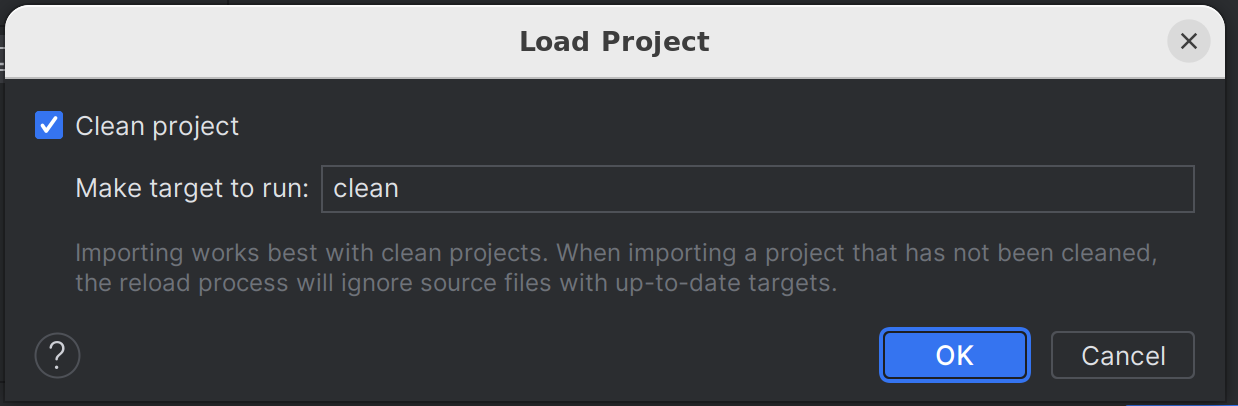
\includegraphics[width=0.5\linewidth]{Pictures/1.png}
    \caption{}
    \label{fig:1}
\end{figure}

Now select the \verb|main.c| file. At the top right corner of the window, click on \verb|Add Configuration| to open the settings for running and debugging. Then, click \verb|Add new...| and \verb|Makefile target|. \\
Fill in the following parameters:\\

\begin{center}
\begin{tabular}{ c c }
 \textbf{Name}: & Makefile  \\ 
 \textbf{Makefile:} & the PATH of the Makefile \\  
 \textbf{Arguments:} & DEBUG=1   
\end{tabular}
\end{center}

\begin{example}{Note}
    You can find the Makefile in the \verb|…/FreeRTOS/Demo/CORTEX_M3_MPS2_QEMU_GCC/Makefile| folder.
\end{example}

\begin{figure}[H]
    \centering
    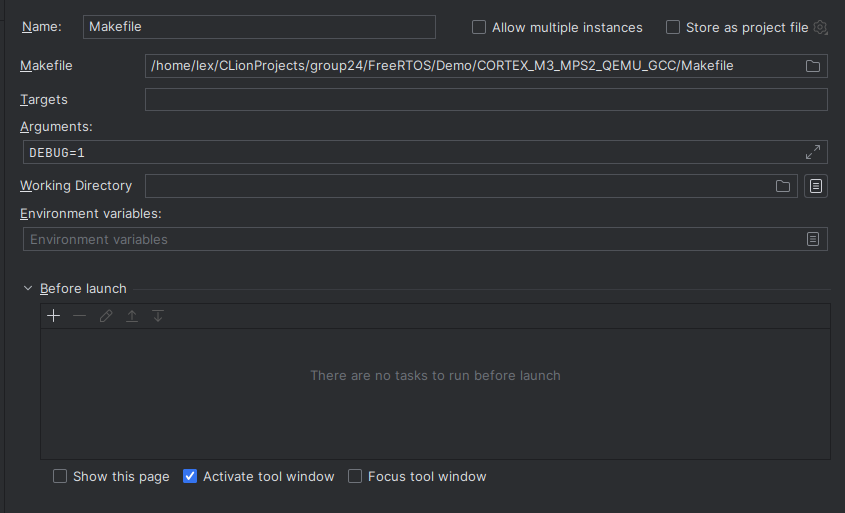
\includegraphics[width=0.7\linewidth]{Pictures/3.png}
    \caption{}
    \label{fig:2}
\end{figure}

Now click \verb|Apply| and then \verb|OK|.\\

It's time to compile: by pressing the \verb|RUN| button (the small triangle) the IDE will automatically run the command
\begin{lstlisting}
make DEBUG=1
\end{lstlisting}
which will use the commands contained in our specified Makefile to do its job. If everything went well, now we should see a folder named \verb|Build| in the root folder of our project. Inside that, we'll find our RTOSDemo.axf file.
\begin{example}{Note}
".axf" is the extension for \textit{ARM Executable Images}. It contains the \textbf{machine code}.
\end{example}
If you're reached this point, the basic setup to compile and run your code on QEMU is complete. Now, let's configure CLion to talk to the debugger.\\
We will now configure an \textbf{Embedded GDB Server} that will do exaclty the same things we did inside our Linux terminal before. First, start by opening the \verb|Edit| menu and select \verb|Edit Configurations...|. Now, click the 'plus' button (top right of the windows that has opened) and select \verb|Embedded GDB Server|. Fill in the following fields:

\begin{center}
\begin{tabular}{ c c }
 \textbf{Name}: & FreeRTOSdemo  \\ 
 \textbf{Executable binary:} & Press on \tcboxverb{...} and then select the \verb|RTOSDemo.axf| file under the \verb|Build| folder. \\
 \textbf{Debugger:} & Bundled GDB multiarch. \\
 \textbf{Download executable:} & \textit{always} \\
 \textbf{'target remote' args:} & tcp:localhost:1234 \\
 \textbf{GDB server:} & \verb|/usr/bin/qemu-system-arm| \\
\end{tabular}
\end{center}

For the \textbf{Target} field, Press the \tcboxverb{Settings} icon, then \tcboxverb{Add target}, and \tcboxverb{Make}. Fill the parameters with the configuration shown in Figure 3. \\  

\begin{figure}[H]
    \centering
    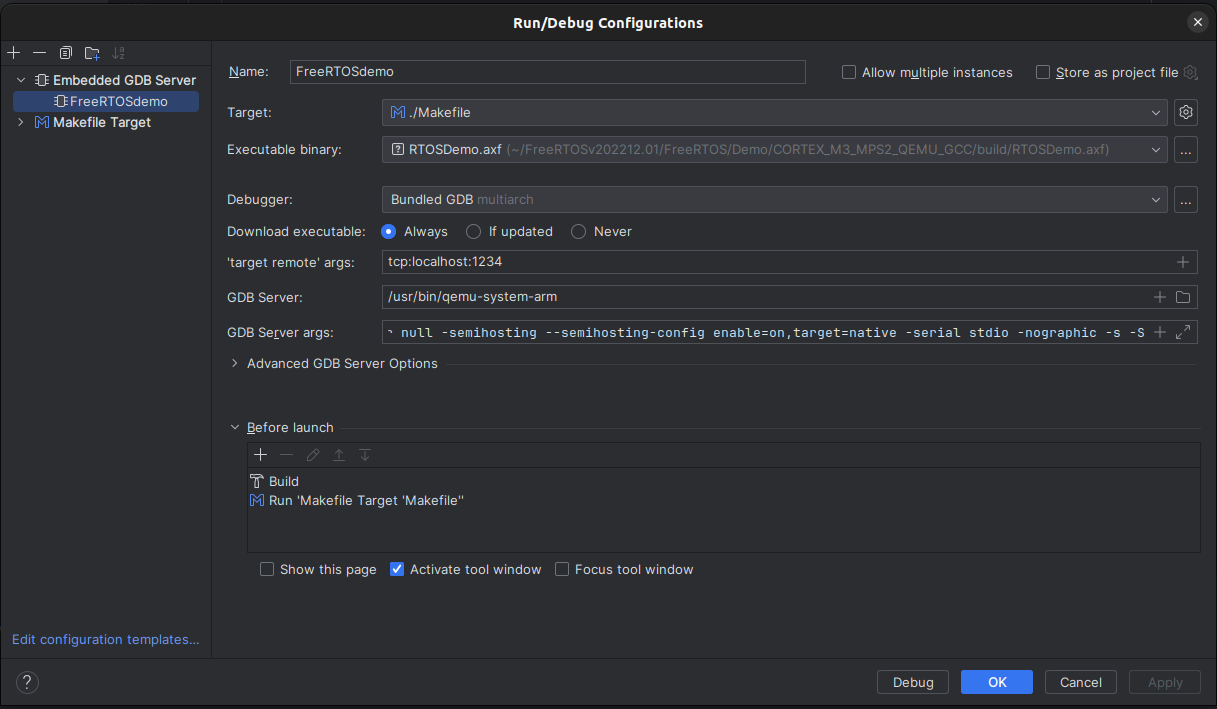
\includegraphics[width=1.0\linewidth]{Pictures/2.png}
    \caption{}
    \label{fig:22}
\end{figure}


For the \textbf{GDB server args} field, write: \verb|-machine mps2-an385 -monitor null -semihosting|\\
\verb|--semihosting-config enable=on,target=native -serial stdio -nographic -s -S|.\\\\
In the Before launch sub-pane, click on the \tcboxverb{+} icon, then choose \tcboxverb{Run another configuration}. Select the Makefile.\\


\begin{Warning}{Warning}
Make sure that as 'Debugger' you have, next to 'Bundled GDB', \textbf{the word \textit{multiarch} in grey} (See Figure 4). If not, select the path of the GDB we have installed previously. If you need help locating it, run the following command in a terminal:
\begin{lstlisting}
which gdb-multiarch
\end{lstlisting}
(default location is \verb|/usr/bin/gdb-multiarch|).

\begin{figure}[H]
    \centering
    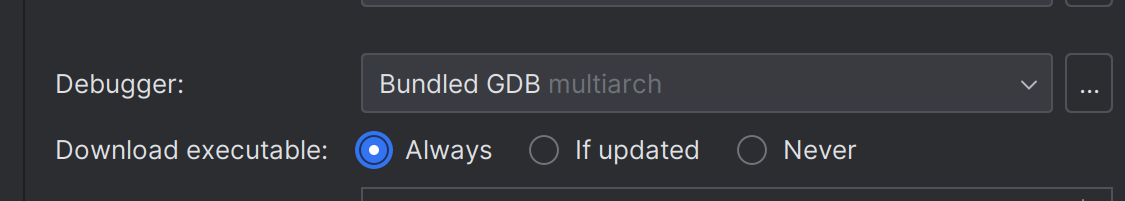
\includegraphics[width=0.5\linewidth]{Pictures/1.5.png}
    \caption{}
    \label{fig:3}
\end{figure} 

\end{Warning}

\begin{example}{Note}
To get the actual path of the GDB Server, run in a terminal the command:
\begin{lstlisting}
which qemu-system-arm
\end{lstlisting}

Default path for us will be \verb|/usr/bin/qemu-system-arm|, because that's the program that will allow us to connect our Demo to the debugger.

\end{example}

We're done here. Click \tcboxverb{Apply} and then \tcboxverb{OK} to return to our code. From now on, every time we will start a debug session from CLion, the IDE will re-compile the executable code using the target Makefile, and run the latest version of the RTSDemofile.axf.\\

Now, let's enable full integration between the IDE and some key data structures in FreeRTOS; this will come particularly in handy because we will be able to navigate into the heap of our simulated OS. In CLion, click \verb|File -> Settings... -> Embedded Development -> RTOS Integration |. Set the \verb|Enable RTOS Integration| checkbox and choose \tcboxverb|FreeRTOS| from the list of options.\\

Now we're really ready to start delving into any code using the debugger. Before doing so, make sure to close all other QEMU instances that you might have started before (the command \verb|killall qemu-system-arm| in a shell should do the trick).

\clearpage
\newpage

\subsection{The FreeRTOS Demo}
Let's find the file \verb|main.c| in our demo project folder (\verb|FreeRTOS/Demo/CORTEX_M3_MPS2_QEMU_GCC/|). \\Since we want to fire up the simple "Blinky" demo, first we need to define  \verb|mainCREATE_SIMPLE_BLINKY_DEMO_ONLY| value to \verb|1|.\\ Let's move on to \verb|main_blinky.c| and take a look at what this piece of code does; basically, it demonstrates of to use a \textit{queue} to pass a value between two tasks (\verb|prvQueueReceiveTask()| function). To handle the succession of events of the exchange, it creates and uses a \textbf{software timer}. \\

\begin{example}{What is a queue?}
Queues are data structures mantained by the OS that work as "buffers"; two tasks that are supposed to exchange information will have access to the same buffer and write on there for the other to see, in a FIFO fashion (do note that the start of the queue is its tail, so if we're depicting the queue as a long "rectangle", we're reading from right to left).\\
\\
When a process writes inside a queue, it will physically make a copy of the data and put it inside; this is particularly useful if we want a task to be able to get the value of one of our variables even after the variable has gone out of scope for the sender. On the other hand, choosing the correct size for a queue, neither too small nor so big that we waste too much space, can be a problem.
\\
\\
Queues can handle various multiprogramming setups: we can configure any number of tasks to read and/or write to a queue, although this also means we will need to take care of "traffic": what do we do if a task wants to read, but the queue is empty? And what if we want to write, but the queue is full? The programmer can specify the maximum time a task will be blocked while waiting for a change before giving up. If the situation solves itself before the timeout(e.g. another task sends to the queue the expected value), then the OS will take care of automatically moving the waiting task to the Ready state.
\end{example}

First, we set the frequency at which the "blinking" will happen:

\begin{lstlisting}
const TickType_t xTimerPeriod = mainTIMER_SEND_FREQUENCY_MS;
\end{lstlisting}

Then, we create the queue using the \verb|xQueueCreate| command:
\begin{lstlisting}
xQueue = xQueueCreate( mainQUEUE_LENGTH, sizeof( uint32_t ) );
\end{lstlisting}

We create two tasks, one called \textit{Rx} and the other called \textit{TX}, to symbolise that they will be the sender and the receiver in the communication. They both have the same \textbf{priority}.
\begin{lstlisting}
// creating task Rx:
xTaskCreate( prvQueueReceiveTask,
             "Rx",
             configMINIMAL_STACK_SIZE,        
             NULL,                           
             mainQUEUE_RECEIVE_TASK_PRIORITY,
             NULL );
// we do pretty much the same for Tx.                      
\end{lstlisting}
We then create an auto-reloading software timer whose period is xTimerPeriod ticks; it will execute the prvQueueSendTimerCallback function everytime it expires:
\begin{lstlisting}
xTimer = xTimerCreate( "Timer",
                        xTimerPeriod,
                        pdTRUE,
                        NULL,
                        prvQueueSendTimerCallback );
\end{lstlisting}
After starting the scheduler, the following events will trigger, each at its set frequency:
- The TX task executes the prvQueueSendTask() function, which sends the value '100' to the xQueue queue every 200 ms.
- Every two seconds, a timer goes off and the handler function that is called writes the value '200' in the xQueue.
- The RX task is put in the ready state by the OS when something arrives in the queue. When it's its turn, it retrieves the message from the xQueue and prints a message.
 
\begin{example}{Scheduling algorithm}
The scheduling algorithm adopted is \textbf{Round Robin} (as you can see from the \verb|configUSE_PREEMPTION| and \verb|configUSE_TIME_SLICING| configuration constants in the \verb|FreeRTOSConfig.h| file). The periods are implemented with the vTaskDelayUntil() function, which puts the task in the blocked state until the specified time has expired.
\end{example}

Now, let's run the program. The final sequence of events is the following:
\begin{lstlisting}
...
[Timer expired] Sent value to queue
[RX task] Message received from software timer
[RX task] Message received from task
[TX task] Sent value to queue
[RX task] Message received from task
[...]
[TX task] Sent value to queue
[RX task] Message received from task
[TX task] Sent value to queue
[Timer expired] Sent value to queue
[RX task] Message received from software timer
[RX task] Message received from task
...
\end{lstlisting}

\begin{example}{Scheduling algorithm}
Do note that the milliseconds stated are only \textit{simulated}, i.e. The code is actually expressed in timer ticks, but it also contains a formula to convert between the number of ticks that have passed and the corresponding "real" time. 
\end{example}

\clearpage
\newpage

\part{Demonstrating FreeRTOS' scheduling algorithms}
\section{The FreeRTOS Scheduler}
The scheduling algorithm applied by FreeRTOS can be tweaked straighforwardly using the \verb|configUSE_PREEMPTION| and \verb|configUSE_TIME_SLICING| configuration constants defined in \verb|FreeRTOSConfig.h|. Whatever the values chosen, the scheduling will be \textbf{priority-based}, and tasks with the same priority will follow the \textbf{Round Robin} schema.\\ As the names suggest, \verb|PREEMPTION| enables the scheduler immediately replace the running task with a new one that has higher priority, while \verb|TIME_SLICING| adds a \textbf{time quantum} to the Round Robin.
\\
\\
In the following pages we present a custom made program that we will run with different configurations as examples.
\subsection{The program}
The program we will use as example is composed of three kinds of tasks: "\textit{server}", "\textit{client setup}", and "\textit{client ping}" (the latter has five different instances, each with a different IP); initially, the client setup task will contact the server to receive five IP configurations from it. After having assigned all the addresses in its pool, the server task quits and an infinite cycle of "pinging" (simulated by printing a message on screen) from the clients starts.\\
To implement this in its base form, each task is given a suitable priority (higher value = higher priority):
\begin{itemize}
\item the task that requests an IP has the highest priority (7)
\item the task that receives the new IP has a low priority (5)
\item the server task that sends out the configuration parameters will have a medium priority (6).
\item the ping tasks have the same priority (1)
\end{itemize}
This way the requests from clients will come before the server does the first reading from the queue. The task that reads the server's reply, on the other hand, is secondary to the server's actions, so we will put it as last.\\
Inside every ping, we call the vTaskDelayUntil() API function; this function puts the task in the \textbf{Blocked state} until its period is over (specified as parameter). This is used to create periodic tasks with a predictable frequence of activation.
\\
\\
Let's focus on the pinging part. A first test, with \verb|configUSE_PREEMPTION = 0| and \verb|configUSE_TIME_SLICING = 0|, yields:
\begin{lstlisting}
Ping sent from 10.0.1.1
Ping sent from 10.0.1.2
Ping sent from 10.0.1.3
Ping sent from 10.0.1.4
Ping sent from 10.0.1.5
[...]
Ping sent from 10.0.1.1
Ping sent from 10.0.1.2
Ping sent from 10.0.1.3
Ping sent from 10.0.1.4
Ping sent from 10.0.1.5
[...]
\end{lstlisting}
The following is the Gantt diagram (CPU clock at 20000000Hz, Tick interrupt at 20000Hz, 100 ticks of delay between two activations of the same task, for all tasks) from the experimental data:

\begin{figure}[H]
    \centering
    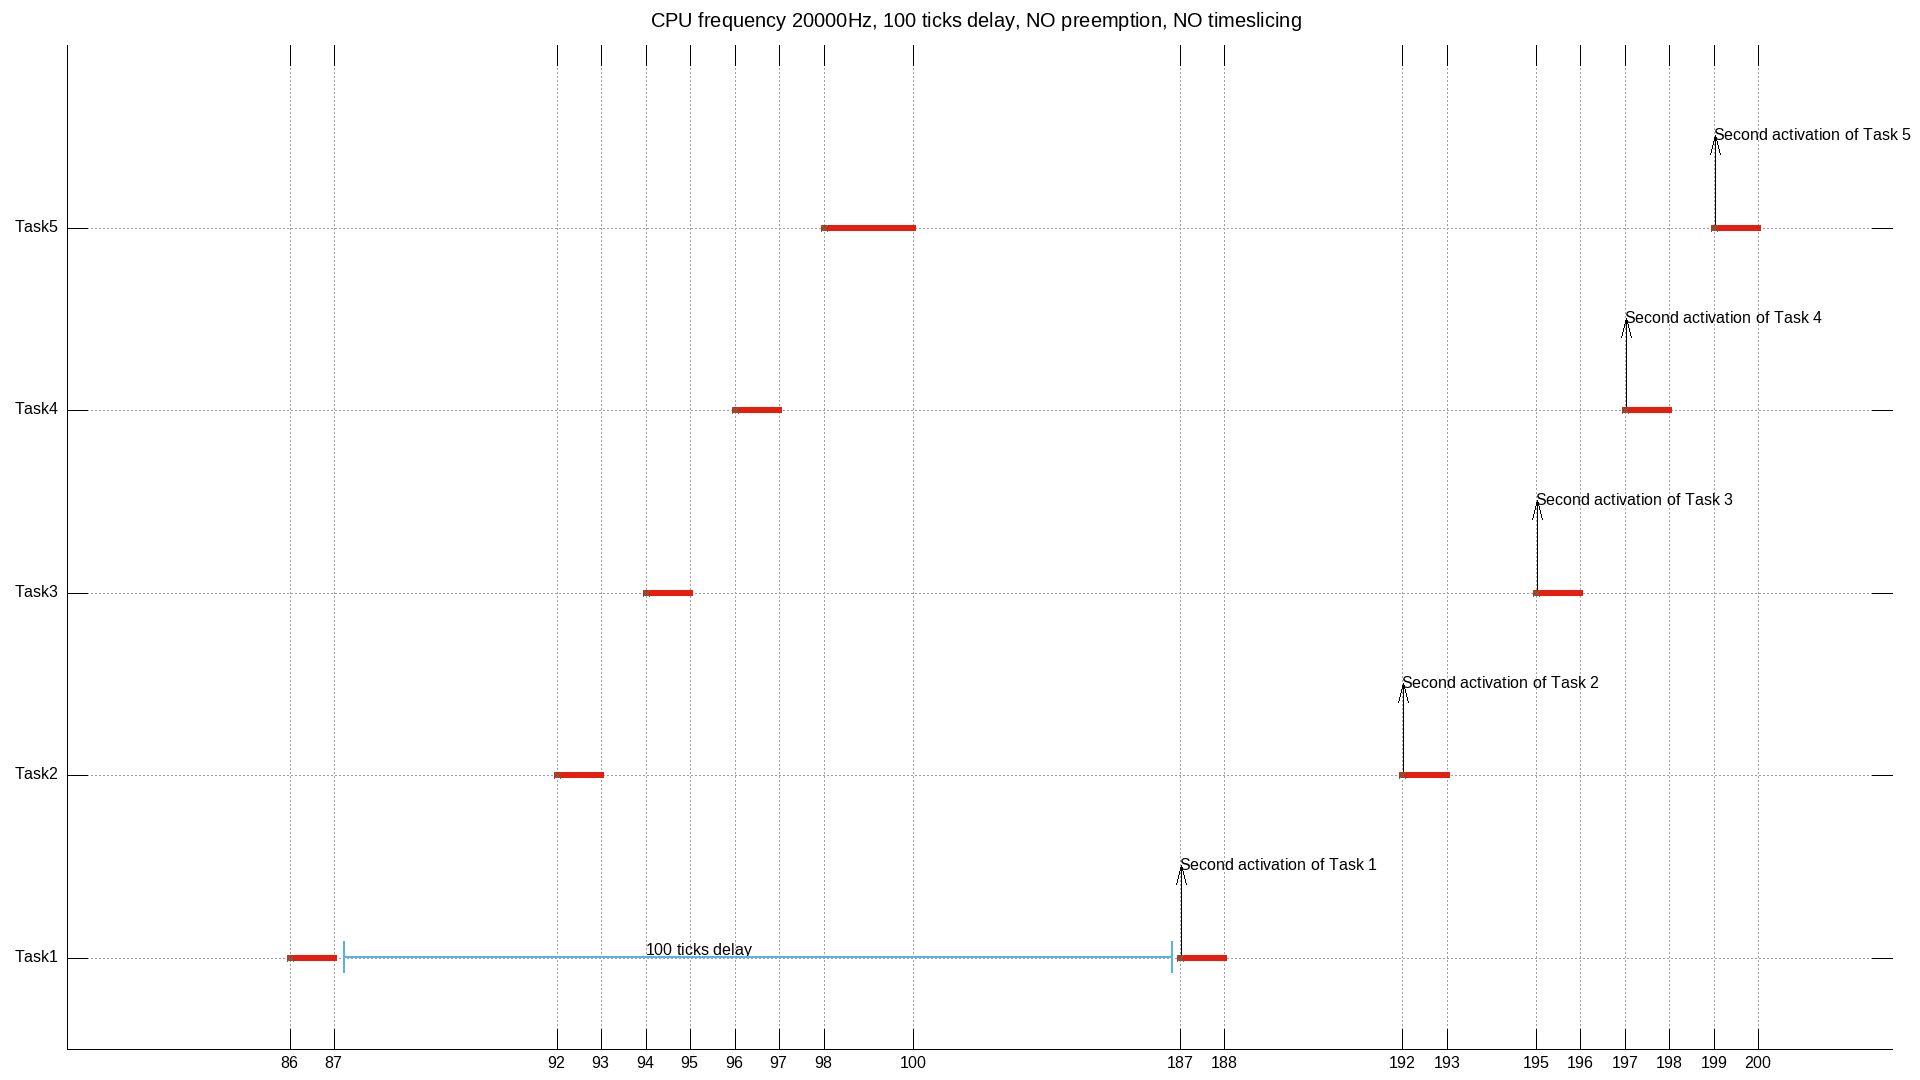
\includegraphics[width=1.0\linewidth]{Pictures/firstGantt.png}
    \caption{}
    \label{fig:4}
\end{figure}

\subsection{Adding preemption}
In this other example, where we've \textbf{added preemption}, tasks 1,3,4 and 5 voluntary enter the blocked state using the vTaskDelayUntil() API function, but task (2) doesn't; instead, it begins an infinite loop with \verb|NULL| instructions. \\ Since we have no set time quantum, and preemption is only applied when a task of higher priority becomes ready (we have none, since all pings have the same priority), the system remains stuck inside client 2's ping.
The sequence of activations will be the following:
\begin{lstlisting}
Ping sent from 10.0.1.1
Ping sent from 10.0.1.2
Ping task from 10.0.1.2 is running...
Ping task from 10.0.1.2 is running...
Ping task from 10.0.1.2 is running...
\end{lstlisting}

If we give task 5 a slighter higher priority than its peers, the following happens:
\begin{lstlisting}
Ping sent from 10.0.1.5
Ping sent from 10.0.1.1
Ping sent from 10.0.1.2
Ping sent from 10.0.1.5
Ping sent from 10.0.1.3
[...]
\end{lstlisting}

During (2)'s infinite loop, (5) becomes active again. Thanks to its higher priority, the scheduler preempts in its favour, breaking 2's loop. After (5) puts itself in the blocked state again (by calling \verb|vTaskDelayUntil()|), the CPU goes to (3) and (4), which have become ready in the meantime...
\\
\\
The following diagrams illustrate the succession of tasks (the numbers in the parenthesis are the content of the ready queue at that moment. Every task is considered ready at the beginning). From this picture, we can deduce FreeRTOS' behaviour with respect to preemption at ready queues:
\begin{itemize}
\item As (2) is preempted because an higher priority task has become ready, it goes at the end of the queue.
\item As (5) becomes active (highest priority), it goes at the top of the queue.
\item All the tasks except for (5) go to the end of the queue when they return ready, because they all have the same priority.
\end{itemize}


\begin{figure}[H]
    \centering
    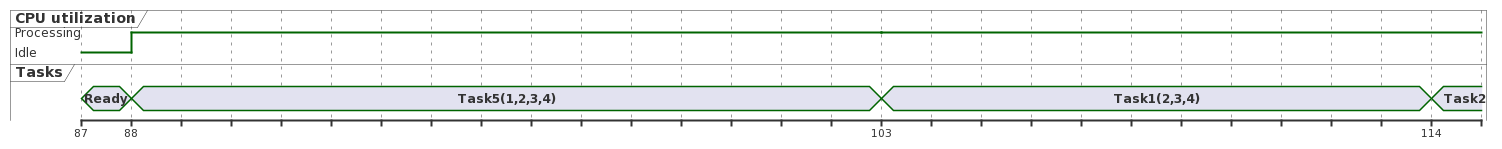
\includegraphics[width=1.0\linewidth]{Pictures/gantt2_1.png}
    \caption{}
    \label{fig:6}
\end{figure}
\begin{figure}[H]
    \centering
    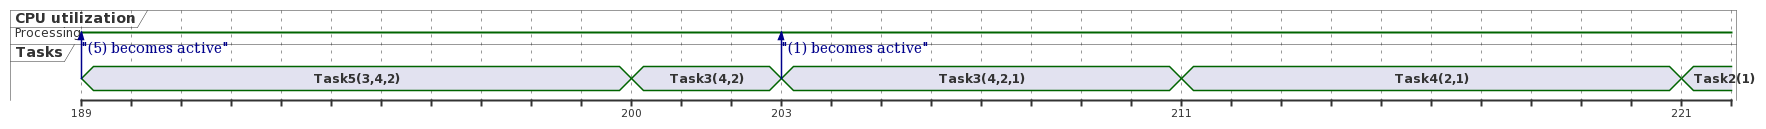
\includegraphics[width=1.0\linewidth]{Pictures/gantt2_2.png}
    \caption{}
    \label{fig:7}
\end{figure}
\begin{figure}[H]
    \centering
    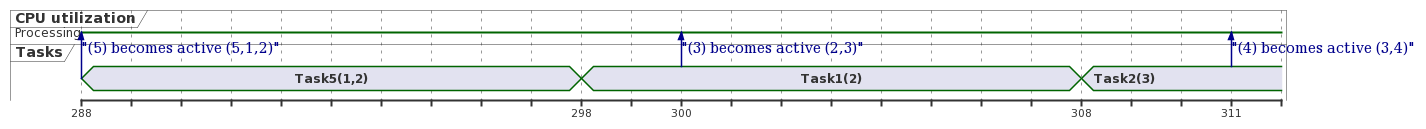
\includegraphics[width=1.0\linewidth]{Pictures/gantt2_3.png}
    \caption{}
    \label{fig:8}
\end{figure}
\begin{figure}[H]
    \centering
    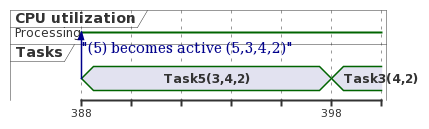
\includegraphics[width=0.3\linewidth]{Pictures/gantt2_4.png}
    \caption{}
    \label{fig:9}
\end{figure}

\section{Adding variety to tasks}
The example showed until now is just a taste of the many combinations of tasks that we could handle. For a more true-to-life experience, at last we add the two new types of tasks the system will handle, and a new revamped version of Ping:
\begin{itemize}
\item In Ping, we've added mathematical computation to the mix, to simulate the actual work the board should do to coordinate a network operation.
\item The second type of task is a "ftp file transfer", where we can follow the passing of time using the CPU thanks to a "progress bar" printed to screen.
\item The third task follows the example of the second one, but this time using the \verb|wget| command.
\end{itemize} 
This is the code we will run the next experiments on, but now let's see how it behaves when we add preemption and we adopt a Round Robin policy for the following set of tasks:
\section{Running example}
To test our new configuration, we used the following parameters (the deadline is supposed relative to the period):

\begin{center}
\begin{tabular}{|c||c|c|c|c|}
\hline 
\rule[-1ex]{0pt}{2.5ex} Task & Priority & Deadline & Period & WCET \\ 
\hline 
\rule[-1ex]{0pt}{2.5ex} Ping Task & 9 & 400 & 600 & 100 \\ 
\hline 
\rule[-1ex]{0pt}{2.5ex} WGET & 8 & 1200 & 1400 & 300 \\ 
\hline 
\rule[-1ex]{0pt}{2.5ex} FTP & 8 & 800 & 1200 & 400 \\ 
\hline 
\end{tabular}
\end{center}

A run with this parameters has given the following results:
\begin{center}
\begin{tabular}{|c|c|c|}
\hline 
\rule[-1ex]{0pt}{2.5ex} Task & Turnaround & Waiting time \\ 
\hline 
\rule[-1ex]{0pt}{2.5ex} Ping & 100 & 0 \\ 
\hline 
\rule[-1ex]{0pt}{2.5ex} WGET & 750 & 450 \\ 
\hline 
\rule[-1ex]{0pt}{2.5ex} FTP & 900 & 500 \\ 
\hline 
\end{tabular} 
\end{center}
\[\begin{bmatrix}
TAT_{avg}=\frac{1760}{3}=583ticks, & WT_{avg}=\frac{950}{3}=316ticks
\end{bmatrix}\]

\begin{figure}[H]
    \centering
    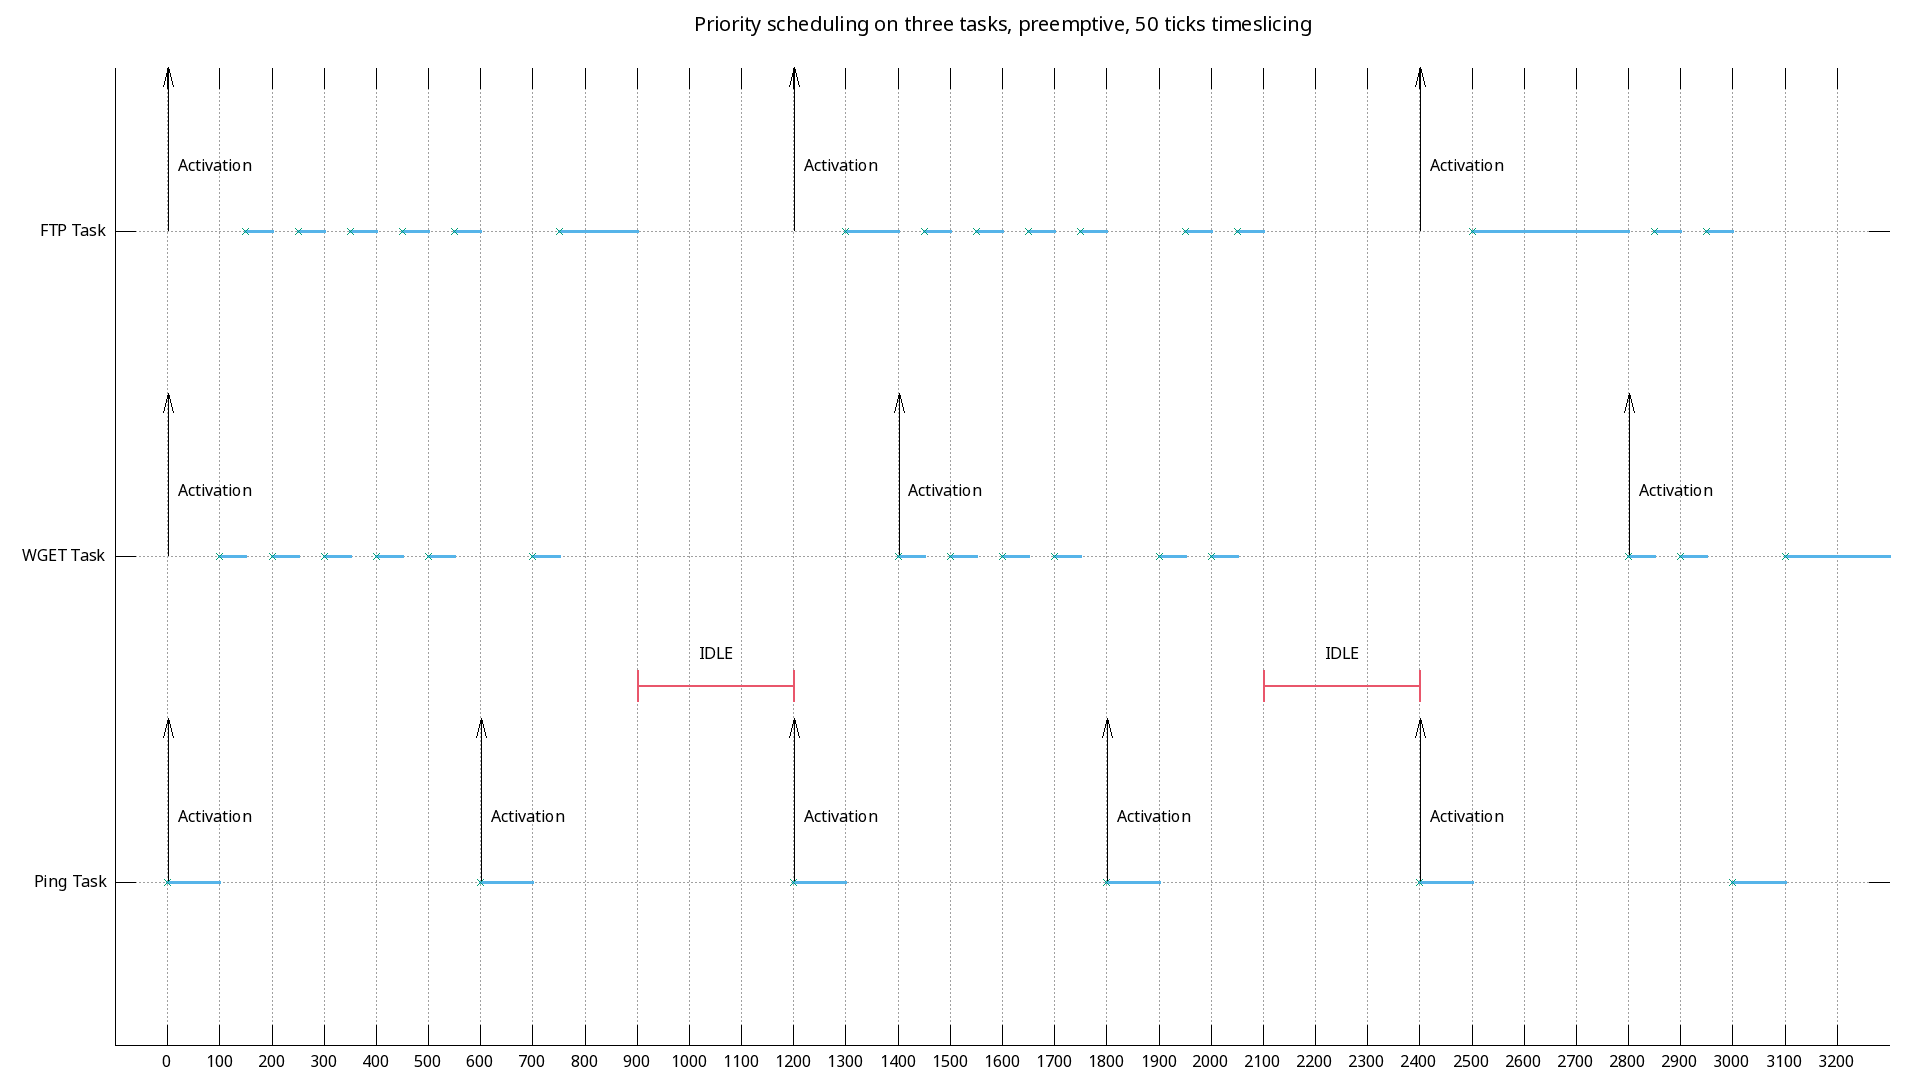
\includegraphics[width=1.0\linewidth]{Pictures/preemRR12feb.png}
    \caption{}
    \label{fig:14}
\end{figure}

From the diagram we observe that FreeRTOS preempts every time the Ping task, the highest priority task, becomes active.
The scheduling is feasible, so we never miss any deadline.
Moreover, the WGET task and the FTP one have the same priority, and, in accordance to the Round Robin algorithm, they each get a fixed time slice before they are preempted to let the other run for the same time, until they are done with their work.
Notice how the first activations of WGET and FTP are forced to resume their work after the second activation of the Ping task is over, and how the latter is able to work for more than its time quantum consecutively only because no other task is ready at the moment.

\newpage

\part{Implementing new Scheduling Algorithms into FreeRTOS}
\section{A first implementation of RMS}
The following part shows the implementation of a new scheduling algorithm, the Rate Monotonic Scheduling, inside FreeRTOS, and the modifications that were made necessary to accommodate such change.\\
\\
As we know, the Rate Monotonic scheduling algorithm schedules periodic tasks by giving them a static priority based on the \textbf{inverse of their period} (the shorter the period, the higher the priority, because it means that it will need to be ready to start again sooner than others). It's also preemptive, so if an higher-priority task becomes active while a lower one is running, the latter will get preempted.
\\
\\
Since FreeRTOS only deals with \textbf{integer} priorities, the code contains a function that "translates" over the [\textit{min priority} \begin{math}\rightarrow\end{math} \textit{max priority}] interval the actual priorities computed according to the definition, which belong to the \begin{math}]0,1[\end{math} interval. The following pseudocode explains how the related C code works:\\

\lstset{language=c}
\begin{lstlisting}
tasks[n];

// we order the tasks[] array using its members' periods (i.e. period(tasks[x]) < period(tasks[x+1]))
orderTasksByPeriod;

//we start assigning a priority that is one step higher than the idle task's priority, since that is supposed to be the lowest one.
nextPriorityToAssign = idle_priority + 1; 


for(all tasks)
{
	changePriorityOfTask(nextPriorityToAssign);
	
	if (the period of the next task is the same as the period of the current one)
	{
		skip increasing the nextPriorityToAssign;
	}
	else
	{
		nextPriorityToAssign++;
	}

\end{lstlisting}

The assigned priorities will be something like (using example data):
\begin{center}
\begin{tabular}{|l|c|}
\hline 
period of a task (in ticks) & priority \\ 
\hline 
399 & 1 \\ 
\hline 
640 & 2 \\ 
\hline 
640 & 2 \\
\hline 
950 & 3 \\ 
\hline 
\end{tabular} 
\end{center}
Albeit simplicistic, this first version of RMS is working as intended; for example, if we create three Ping tasks with the following characteristics
\\
\begin{center}
\begin{tabular}{|c|c|c|}
\hline 
Task & Period (ticks) & WCET (ticks) \\ 
\hline 
T1 & 37 & 10\\ 
\hline 
T2 &  43 & 10\\ 
\hline 
T3 & 47 & 10\\ 
\hline 
\end{tabular} 
\end{center}
And we compile the Gantt diagram of the actual execution, using experimental data:
\begin{figure}[H]
    \centering
    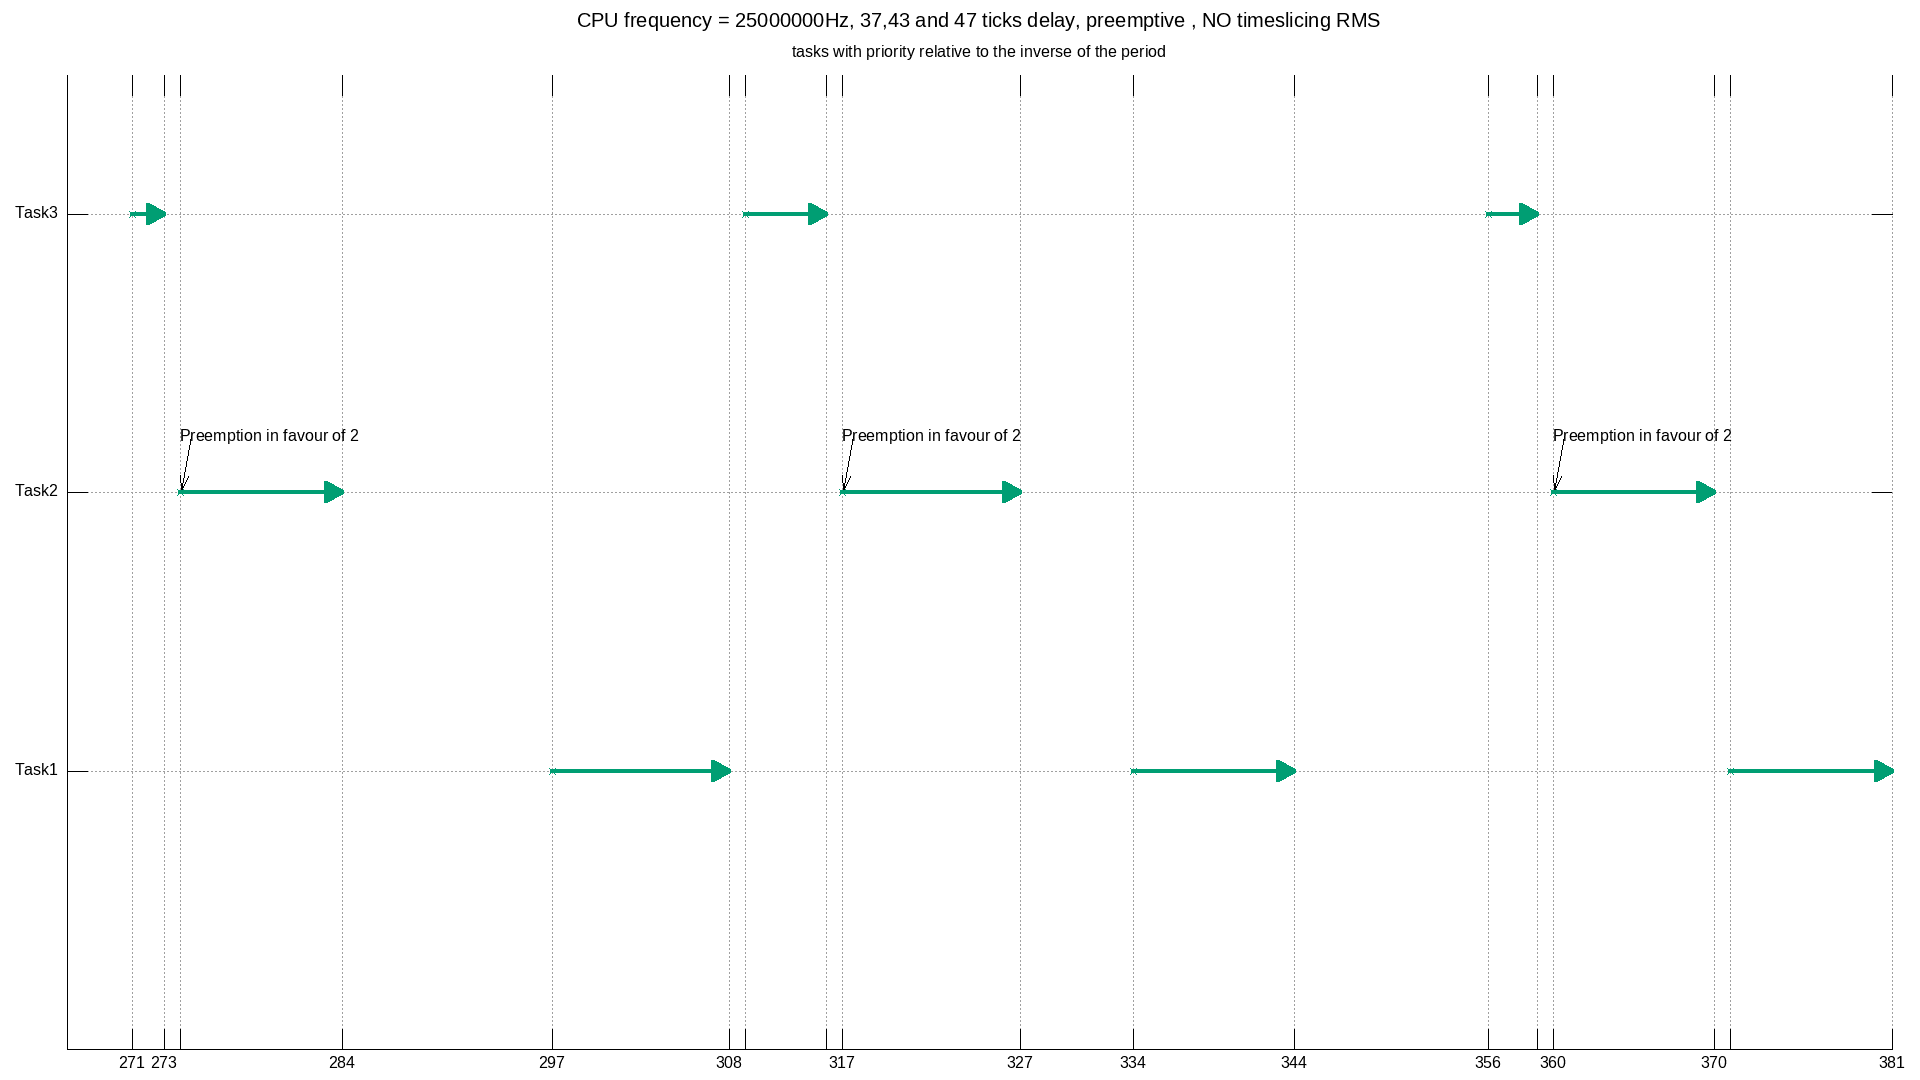
\includegraphics[width=1.0\linewidth]{Pictures/RMSgantt.png}
    \caption{}
    \label{fig:10}
\end{figure}
We can confirm that the tasks are \textbf{activating respectively every 37, 43 and 47 ticks}, and using the CPU each for 10 ticks (again, when not preempted first) before putting themselves in the blocked state.
We also showed that the tasks have been \textbf{ordered according to their priority}: Task2 takes precedence on all the others because it has the shortest period, while T1 runs with the least. \begin{example}{Note}
Task3's periods are less consistent than the other two tasks' because it's often preempted before it has the chance to set its next wake-up time using \verb|vTaskDelayUntil()|.
\end{example}

\section{A more elaborate RMS implementation}
The last implementation tried to make do with the structures and methods of FreeRTOS by, essentially, just hijacking the function to create tasks and delaying it until we have a full view of all the tasks that are supposed to run in the system, and then call it again "under the hood" with modified parameters.
After carefully studying the original \verb|task.c| code, we've delved into creating custom OS structures such a custom Task Control Block for out RMS-controlled tasks.

\begin{example}{Note}
In our effort, we tried to remain truthful to the original developers' code style and data types, using the official \href{https://www.freertos.org/FreeRTOS-Coding-Standard-and-Style-Guide.html}{Style Guide}.
\end{example}

\lstset{language=c}
\begin{lstlisting}
typedef struct tskCustomTaskControlBlock{
   
    // [...] original TCB members

    TickType_t xLastWakeTime;       // Parameter to track the last wake time of the task
    TickType_t xArrivalTime;        // Arrival time of the task
    TickType_t xPeriod;             // Period of the task
    TickType_t xWCET;               // Worst Case Execution Time
    TickType_t xTimeSpent;          // Time elapsed since task start
    TickType_t xDeadline;           // Deadline of the task

}cTCB_t;

\end{lstlisting}
With this we will have a way, built-in into each task's core, to always keep track of critical parameters for our scheduling decisions.

\lstset{language=c}
\begin{lstlisting}
void vPeriodicTaskCreate( // [...] original TaskCreate parameters
							            TaskHandle_t *pxTaskHandle,
                          TickType_t xArrivalTime,
                          TickType_t xPeriod,
                          TickType_t xDeadline,
                          TickType_t xWCET
					            	)
{
	// we start as normal:
    cTCB_t *pxTCB;
    pxTCB = pvPortMalloc(sizeof( cTCB_t ));
    // [...]
    // ... then we assign the new data to their field inside our custom TCB:
    pxTCB->xArrivalTime = xArrivalTime;
    pxTCB->xPeriod = xPeriod;
    pxTCB->xWCET = xWCET;
    // [...]

}

\end{lstlisting}

Now that we've created a new control structure, and we've succesfully initialized it, we need to modify how we call the scheduler to go along with the new information; to do it, we're adding a new function, \verb|vTaskStartRealTimeScheduler()|, which will take care of the initialization of RMS-related fields and then, before exiting, it will call the canonical \verb|vTaskStartScheduler()| to tie all out changes together with what is already a part of FreeRTOS:
\begin{lstlisting}
void vTaskStartRealTimeScheduler(){
    #if( configENABLE_RM == 1 )			//custom config parameter definition in freeRTOSconfig.h
      prvAssignPriorityRMS();
    #endif

    prvCallTaskCreate();			// use xTaskCreate to submit a task to FreeRTOS' scheduler
    xStartTime = xTaskGetTickCount();
    vTaskStartScheduler();			//start FreeRTOS' scheduler
}
\end{lstlisting}

\begin{example}{Note}
We've declared some static global variables at the top of the file (\verb|RealTimeScheduler.c|):
\begin{lstlisting}
static TickType_t xStartTime = 0;       // Time elapsed since the scheduler started
static BaseType_t xIdleFlag = 0;        // Flag to know if Idle Task is active.

#if( configENABLE_RM == 1 )
    static List_t xTASK_List;
    static List_t *pxTASK_List = NULL;
#endif
\end{lstlisting}
Where \verb|xTASK_List| is a list of all the custom TCBs we've created, and \verb|*pxTASK_List| points to the beginning of said list.\\
\end{example}
\newpage
At last, let's dive in depth in the most important part of the implementation, the actual priority assigning behaviour defined in \verb|prvAssignPriorityRMS()|:

\begin{lstlisting}
        static void prvAssignPriorityRMS() {
           [...]
        current priority = highest priority -1;
        
		while( head of TCB list != tail of TCB list )
		{
                priority of current TCB = current priority;
                current priority--;

                current TCB = next TCB in list;
            }
            }
\end{lstlisting}
\begin{example}{Note}
In this code we're just assigning priorities from higher to lower at each step, because the list is already sorted by ascending periods as a result of calling \verb|prvInitialiseTCBItemRMS(cTCB_t *pxTCB)| (more specifically, the \verb|listSET_LIST_ITEM_VALUE( &pxTCB->pxTCBItem, pxTCB->xPeriod);| line sets the period field of a TCB as the field that the sorting is done on).\\\\ 
FreeRTOS' lists are not "normal" C lists: they have been enhanced to handle TCB members specifically. For example, each member of a list must be given a reference to the list it is part of (its \textit{container}). \\An example of how we used such lists is inside \verb|vInitScheduler()|: first we initialize the Task List, and then we assign a global variable with the pointer to its beginning.
\begin{lstlisting}
void vInitScheduler(){
    #if( configENABLE_RM == 1)
        vListInitialise( &xTASK_List );     // Initialization of Task List
        pxTASK_List = &xTASK_List;          // Assigning the global variable
    #endif
}
\end{lstlisting}
For each custom TCB we need to initialize it as a list item and add it to it using \verb|prvInitialiseTCBItemRMS( cTCB_t *pxTCB ) |:
\begin{lstlisting}
    static void prvInitialiseTCBItemRMS( cTCB_t *pxTCB ) {
    
        /* vListInitialiseItem initializes the container to null so the item
         * does not think that it is already contained in a list*/
        vListInitialiseItem( &pxTCB->pxTCBItem );
        
        /* The owner of a list item is a pointer to the object (usually a TCB) that holds the list item's contents */
        listSET_LIST_ITEM_OWNER( &pxTCB->pxTCBItem, pxTCB );
        
        listSET_LIST_ITEM_VALUE( &pxTCB->pxTCBItem, pxTCB->xPeriod);

        /* Insert the Item in the Task List */
        vListInsert( pxTASK_List, &pxTCB->pxTCBItem );
    }

\end{lstlisting}
\end{example}
\newpage
Now, we present the content of \verb|prvCallTaskCreate|: this function calls FreeRTOS' xTaskCreate to submit our tasks to FreeRTOS' scheduler, one by one, reading from our TCB list:
\begin{lstlisting}
static void prvCallTaskCreate(){
    [...]
    while( pxTCB_Pointer != pxTCB_Tail ){
        pxTCB = listGET_LIST_ITEM_OWNER( pxTCB_Pointer );
        xTaskCreate( prvPeriodicTaskMaster, //pointer to the code to execute during the task
                     pxTCB->pcName,
                     pxTCB->ulStackDepth,
                     pxTCB->pvParameters,
                     pxTCB->xPriority,
                     pxTCB->pxTaskHandle);
        pxTCB_Pointer = listGET_NEXT( pxTCB_Pointer );
    }
}
\end{lstlisting}
\begin{Warning}{Very important}
Notice that every task we're creating is technically instructed to execute \textbf{one function in all cases}: \verb|prvPeriodicTaskMaster|.
The \verb|prvPeriodicTaskMaster| will be the core of our most complex decision taking, because it's the \textit{wrapper function} that will take care of selecting which Task function code to run (the ping, the WGET or the FTP) every time.

\begin{lstlisting}
static void prvPeriodicTaskMaster( void *pvParameters )
{
    // We retrieve the TCB of the task we want to run:
    cTCB_t *pxTask = prvGetTCBFromListByHandleRMS(xCurrentTaskHandle);
    
    for ( ; ; )
    {
        if (IdleFlag == 1)
        {
         printf "IDLE";
         IdleFlag = 0.
        }
    
        else 
        {
        // Now we call the task function code specified in the TCB (WGET, Ping or FTP)
        pxTask->pxTaskCode( pvParameters );
        
        printf(info on the running task);
        [...]
        printf( name, length of this CPU burst 	and WCET);
 		
        putTaskInBlockState(TCB->period);
        }        
    }
}

\end{lstlisting}
\end{Warning}

\subsection{Running example}
This is the final result for our three tasks:
\begin{center}
\begin{tabular}{|c||c|c|c|}
\hline 
\rule[-1ex]{0pt}{2.5ex} Task & Period & Arrival time & WCET \\ 
\hline 
\rule[-1ex]{0pt}{2.5ex} Ping Task & 600 & 0 & 100 \\ 
\hline 
\rule[-1ex]{0pt}{2.5ex} WGET & 1400 & 0 & 300 \\ 
\hline 
\rule[-1ex]{0pt}{2.5ex} FTP & 1200 & 0 & 400 \\ 
\hline 
\end{tabular}
\end{center}

The schedule is theoretically feasible:
\[\bigg(\frac{1}{6}+1\bigg)\cdot\bigg(\frac{3}{14}+1\bigg)\cdot\bigg(\frac{1}{3}+1\bigg)\le 2\]

The turnaround and waiting time for each task (in ticks) is:
\begin{center}
\begin{tabular}{|c|c|c|}
\hline 
\rule[-1ex]{0pt}{2.5ex} Task & Turnaround & Waiting time \\ 
\hline 
\rule[-1ex]{0pt}{2.5ex} Ping & 100 & 0 \\ 
\hline 
\rule[-1ex]{0pt}{2.5ex} WGET & 800 & 600 \\ 
\hline 
\rule[-1ex]{0pt}{2.5ex} FTP & 500 & 100 \\ 
\hline 
\end{tabular} 
\end{center}
\[\begin{bmatrix}
TAT_{avg}=\frac{1500}{3}=500ticks, & WT_{avg}=\frac{700}{3}=233ticks
\end{bmatrix}\]

\begin{figure}[H]
    \centering
    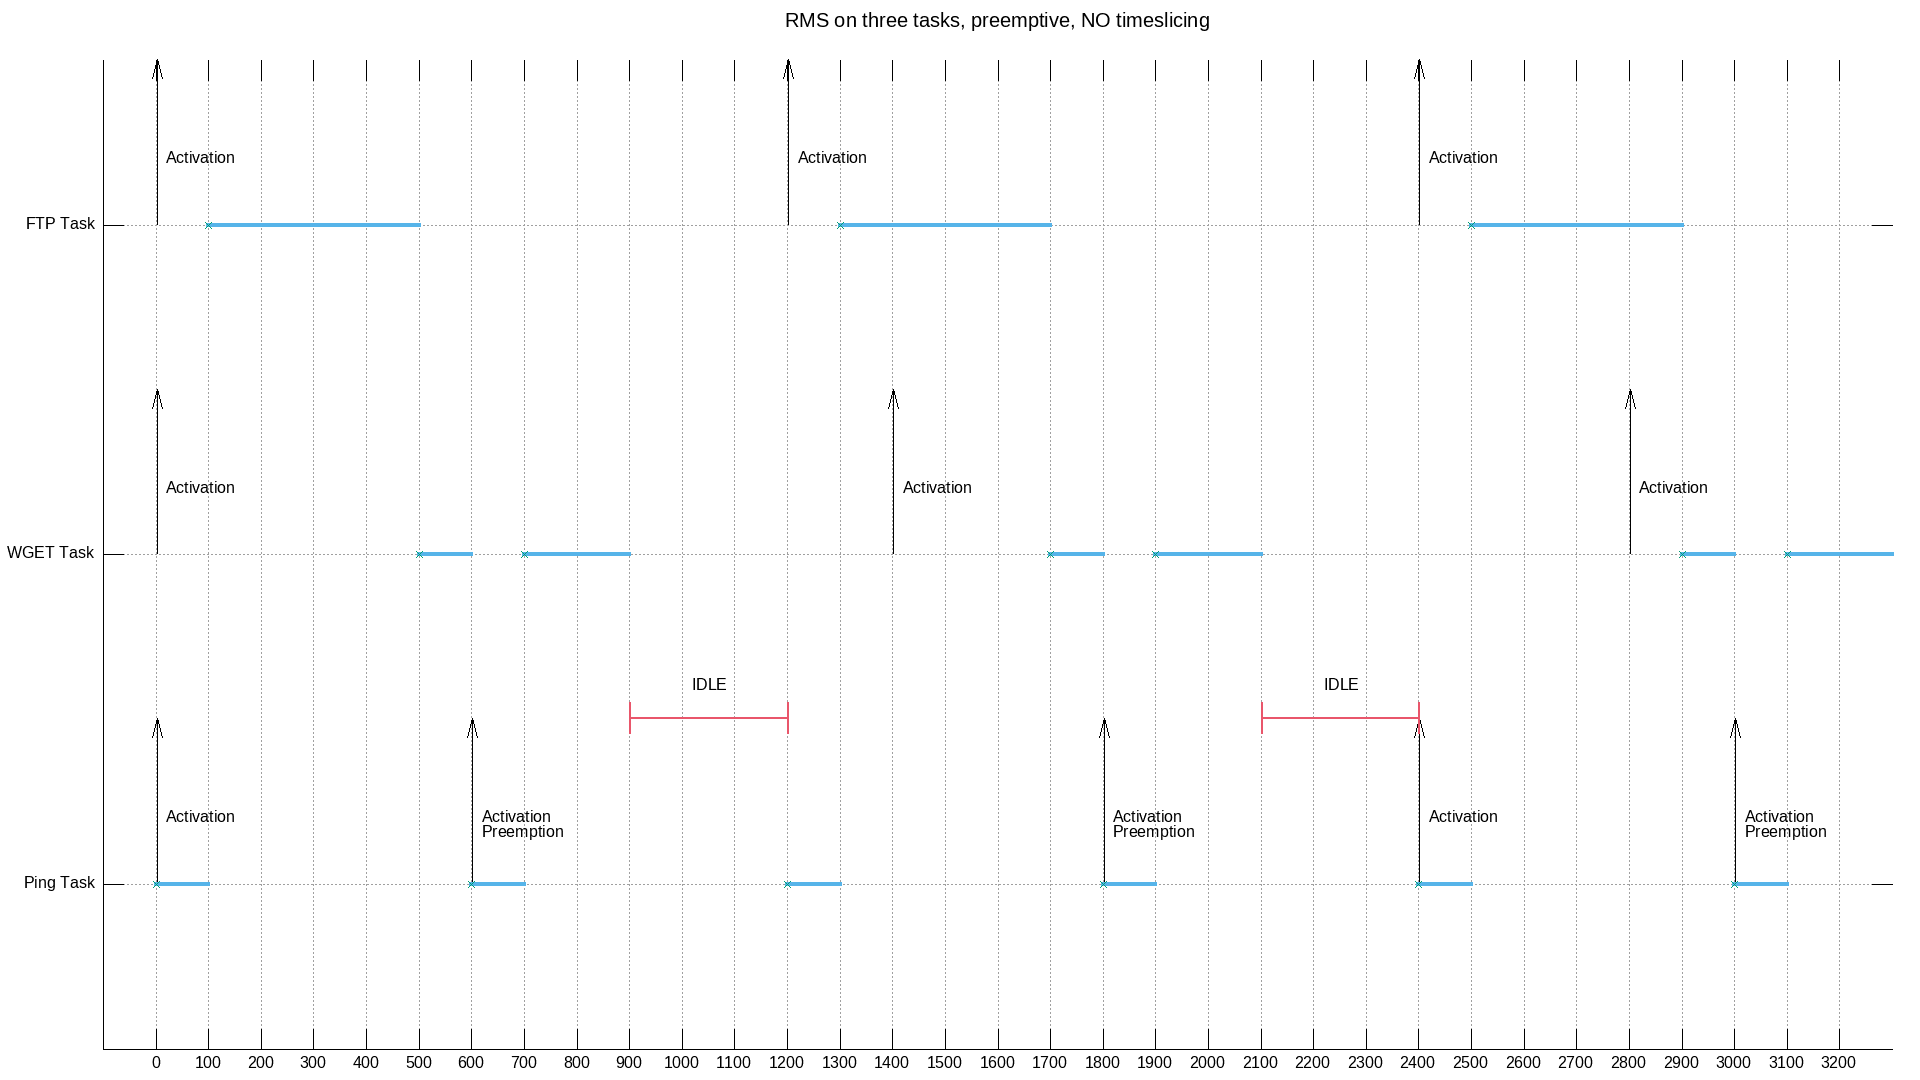
\includegraphics[width=1.0\linewidth]{Pictures/RMSgantt2.png}
    \caption{}
    \label{fig:11}
\end{figure}
\newpage
\newpage
\section{Implementing Earliest Deadline First}

Earliest Deadline First is another scheduling algorithm that is particularly suited for periodic tasks. We built upon what we learned while working with RMS to implement EDF too.
\\\\
The most challenging aspect of this implementation was going from computing priorities once to making \textbf{decisions every time a scheduling event occurs}, such as when a task is put in the blocked state or when a task becomes active again after some waiting.
The second major problem was adding the logic behind scanning the ready queue and \textbf{finding the process closest to its deadline at any moment}.
\\
\begin{itemize}
\item The Custom TCB was improved with the \verb|TickType_t xAbsDeadline;| field, to keep the result of the kernel's computation of the current deadline for a process.
\item We implemented new functions to adapt to the TCB changes, such as\verb|prvGetTCBFromListByHandleEDF| and \verb|prvInitialiseTCBItemEDF|.
\item The number and nature of the tasks list had to be modified too: we added a temporary task list (\verb|xTASK_List_tmp|) that will work with the original one to deal with changes to the scheduling order.
\item the creation of a new periodic task has the added complication of initializing the current deadline, i.e. the system time the task will need to be completed by. We do it by adding together the task's arrival time and the set time limit (\verb|xDeadline|):
\lstset{language=c}
\begin{lstlisting}
void vPeriodicTaskCreate(){

    [...]
    #if( configENABLE_EDF == 1 )
    pxTCB->xAbsDeadline = pxTCB->xDeadline + pxTCB->xArrivalTime + xStartTime;
    prvInitialiseTCBItemEDF( pxTCB );
    #endif
		[...]

}
\end{lstlisting}
\item The \verb|vApplicationTickHook| function is updated to adapt to the TCB changes and the presence of the custom EDF scheduler. 
\item The \verb|prvPeriodicTaskMaster| was, predictably, one of the most worked on functions. We analyze its changes in the following subsection.
\item The scheduler is now a \textit{EDF Scheduler}, which is a task that executes a function called \verb|prvSchedulerEDFCode|:
\begin{lstlisting}
static void prvSchedulerEDFCode(){
        for( ; ; ){
        	// Update priorities
            prvCheckPrioritiesEDF();
            // Give the signal to unblock the next task in line
            ulTaskNotifyTake( pdTRUE, portMAX_DELAY );
        }
    }
\end{lstlisting}
\end{itemize}
\subsection{Changes related to PeriodicTaskMaster}
\verb|prvPeriodicTaskMaster()| has been though major changes, such as a new \verb|printf| that accounts for new information (the task's deadline), and the \verb|prvNotifySchedulerEDF()| function, which we need to \textbf{notify the scheduler} that the current task is done running, so it's the right time to \textbf{update its priorities}.

\lstset{language=c}
\begin{lstlisting}
static void prvPeriodicTaskMaster( void *pvParameters ){
    TaskHandle_t xCurrentTaskHandle = xTaskGetCurrentTaskHandle();
   [...]
    #elif( configENABLE_EDF == 1 )
        cTCB_t *pxTask = prvGetTCBFromListByHandleEDF(xCurrentTaskHandle);
    #endif

    [...]

    for ( ; ; )
    {
        [...]
        #if( configENABLE_EDF == 1)
            prvNotifySchedulerEDF();
            printf(Tick Count, Task name, last Wake Time, Abs deadline, Priority);
        #endif
        
        [...]
        
       //run the current task's code

       #if( configENABLE_EDF == 1 )
           pxTask->xAbsDeadline = pxTask->xDeadline + pxTask->xLastWakeTime + pxTask->xPeriod;
           // Notify scheduler that the task has been executed and update priorities:
            prvNotifySchedulerEDF();
       #endif
       
     vTaskDelayUntil( &pxTask->xLastWakeTime, pxTask->xPeriod );


    }
}
\end{lstlisting}
The \verb|prvNotifySchedulerEDF| function is another new addition to our code. The function is used to first notify the EDF Scheduler to update the priorities, and then request a context switch to the highest priority task. 

\lstset{language=c}
\begin{lstlisting}
  static void prvNotifySchedulerEDF(){
        BaseType_t xHigherPriorityTaskWoken;
        // Notify the scheduler task to run its code again. 
        vTaskNotifyGiveFromISR( xSchedulerEDFHandle, &xHigherPriorityTaskWoken );
        // Request a context switch to the higher priority task returned by the scheduler
        portEND_SWITCHING_ISR( xHigherPriorityTaskWoken );
    }
\end{lstlisting}
\verb|prvNotifySchedulerEDF| is called inside the \verb|PeriodTaskMaster| code after the current Ping/WGET/FTP function (\verb|pxTaskCode|) returns; this will in turn alert the scheduler task (whose handle is \verb|xSchedulerEDFHandle|) that we should temporarily block \verb|PeriodTaskMaster| while we update our priorities; this is done by calling \verb|vTaskNotifyGiveFromISR| with a flag parameter, \textit{xHigherPriorityTaskWoken}, that is set to 'false'.
After the update, the scheduler will then set the flag to 'true' again, acting like a "green semaphore" for \verb|PeriodTaskMaster|.

\subsection{Assigning priorities}
The \verb|prvSetEDF| method takes care of initializing the priorities for the first run of the EDF scheduler. The logic behind it is, obviously, giving higher priority of tasks that have a deadline closer in time. We do this by just traversing the TCB list and setting the priorities from highest to lowet value, since the list is already sorted by ascending deadlines.
\begin{lstlisting}
    /* Assign priorities while traversing the Sorted List */
    static void prvSetEDF(){
        cTCB_t *pxTCB;
        [...]

        while( currentTCB_Pointer != pxTCB_Tail ){
            currentTCB = listGET_LIST_ITEM_OWNER( currentTCB_Pointer );
            
            currentTCB->xPriority = xHighestPriority;
            xHighestPriority--;

            currentTCB_Pointer = listGET_NEXT( pxTCB_Pointer );
        }
    }
\end{lstlisting}
Now, let's see how these priorities are \textbf{changed on the fly} based on their newly computed absolute deadlines:
\begin{lstlisting}
/* Assign new priorities to tasks based on their new absolute deadlines */
    static void prvCheckPrioritiesEDF(){
        [...]

        currentTCB_Pointer = listGET_HEAD_ENTRY( pxTASK_List );
        const ListItem_t currentTCB_Tail = listGET_END_MARKER( pxTASK_List );
        
        while( traversing TCB list ){
           [...]

            // Sort again the list by the updated absolute deadlines
            listSET_LIST_ITEM_VALUE( currentTCB_Pointer , currentTCB->xAbsDeadline );

            // We keep a temporary list while updating the pxPrevious fields of each list member to make it point to the correct previous TCB in the list
            currentTCB_Pointer_tmp = currentTCB_Pointer;
            currentTCB_Pointer = listGET_NEXT( currentTCB_Pointer );
            uxListRemove( currentTCB_Pointer->pxPrevious );
            
			// Adding the current TCB to the list
            vListInsert( pxTASK_List_tmp, currentTCB_Pointer_tmp );
        }

        swap(currentTCBlist,tempTCBlist);
        
        // Update priorities based on new task order, from highest to lowest, while traversing the ordered TCB list
        
           currentPriorityToAssign = SCHEDULER_PRIORITY - 1;
       	[...]
        while( traversing TCB list ){
   	[...]
            currentTCB->xPriority = currentPriorityToAssign;
            
            // Set the new updated priority to the target task
            vTaskPrioritySet( currentTCB->pxTaskHandle, currentTCB->xPriority );
            
            currentPriorityToAssign--;
            [...]
        }
    }

\end{lstlisting}

\section{Running example}
To test our new configuration, we used the following parameters (the deadline is supposed relative to the period):
\begin{center}
\begin{tabular}{|c||c|c|c|c|}
\hline 
\rule[-1ex]{0pt}{2.5ex} Task & Start Time & Deadline & Period & WCET \\ 
\hline 
\rule[-1ex]{0pt}{2.5ex} Ping Task & 0 & 400 & 600 & 100 \\ 
\hline 
\rule[-1ex]{0pt}{2.5ex} WGET &  0 & 800 & 1200 & 400 \\ 
\hline 
\rule[-1ex]{0pt}{2.5ex} FTP & 0 & 1200 & 1400 & 300 \\ 
\hline 
\end{tabular}
\end{center}

The turnaround and waiting time for each task (in ticks) is:
\begin{center}
\begin{tabular}{|c|c|c|}
\hline 
\rule[-1ex]{0pt}{2.5ex} Task & Turnaround & Waiting time \\ 
\hline 
\rule[-1ex]{0pt}{2.5ex} Ping & 100 & 0 \\ 
\hline 
\rule[-1ex]{0pt}{2.5ex} WGET & 900 & 600 \\ 
\hline 
\rule[-1ex]{0pt}{2.5ex} FTP & 500 & 100 \\ 
\hline 
\end{tabular} 
\end{center}
\[\begin{bmatrix}
TAT_{avg}=\frac{1500}{3}=500ticks, & WT_{avg}=\frac{700}{3}=233ticks
\end{bmatrix}\]

\begin{figure}[H]
    \centering
    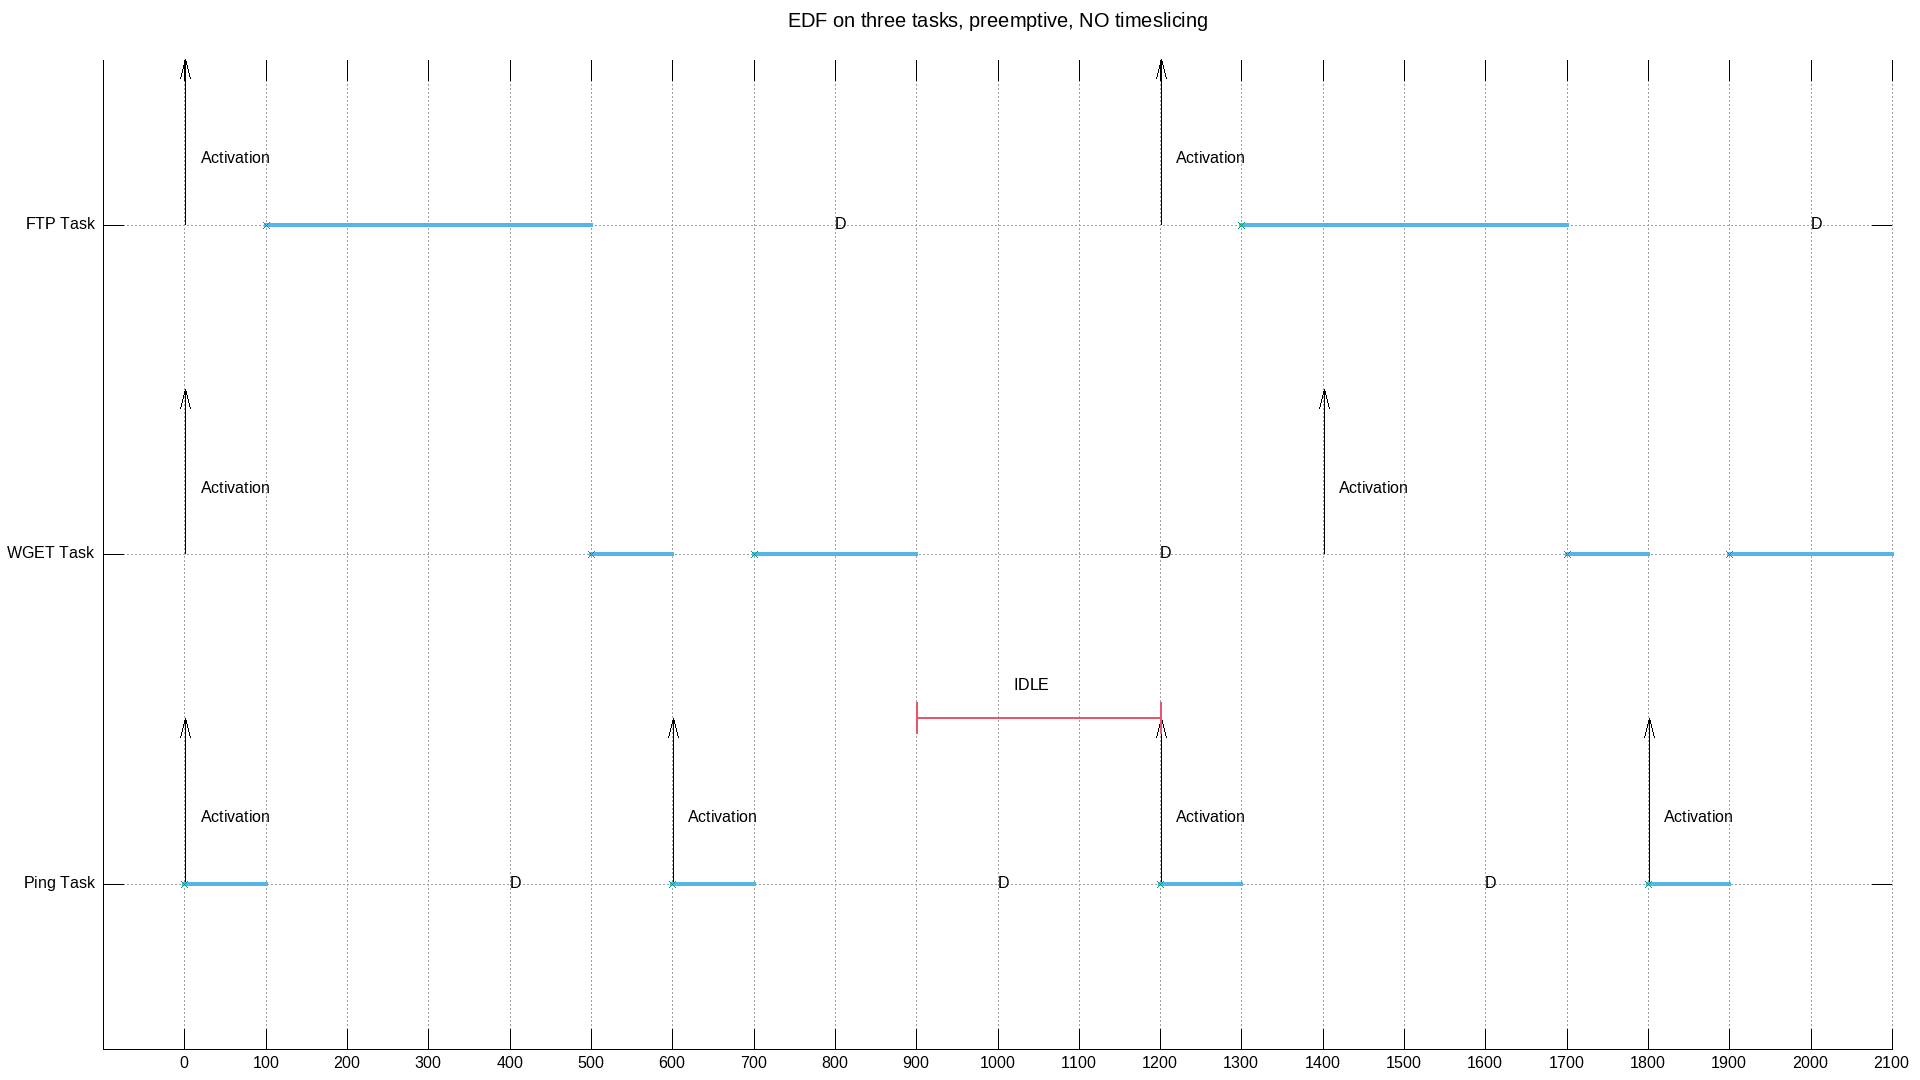
\includegraphics[width=1.0\linewidth]{Pictures/EDFgantt.png}
    \caption{}
    \label{fig:12}
\end{figure}
\newpage
\section{Adding aperiodic tasks: Polling Servers implementation}
In this last section we present a solution to deal with aperiodic tasks, namely the Polling Servers algorithm.
As before, we need to make changes throughout the code:
\begin{itemize}
\item Our custom TCB has two more fields: \verb|xPS|, \textbf{a flag that signals that a task is a Polling Server}, and \verb|xBudgetPS|, \textbf{the budget assigned to said Server}. 
\begin{lstlisting}
typedef struct tskCustomTaskControlBlock{
 [...]

    #if( configENABLE_APERIODIC == 1)
        BaseType_t xPS;             // Flag for Polling Server
        TickType_t xBudgetPS;       // Budget of Polling Server
    #endif

    [...]

}cTCB_t;

\end{lstlisting}
\item We define yet another type of TCB: \verb|tskAperiodicTaskControlBlock|, to contain all information needed for its scheduling:
\begin{lstlisting}
 typedef struct tskAperiodicTaskControlBlock{
       [...]
        TickType_t xWCET;               // Worst-Case-Time-Execution
        ListItem_t pxTCBAItem;          // Item object for task list (owner)
        BaseType_t xArrival;            // Arrival Time used as key for sorting the queue
    } cTCBA_t;
\end{lstlisting} 
\item The custom TCB's fields are first populated by \verb|vAperiodicTaskCreate|. Notice how, each time a new aperiodic task comes, we assign the next value of an integer counter to keep track of the relative order of arrival of this kind of tasks:
\begin{lstlisting}
    void vAperiodicTaskCreate( ... ){
        xArrival++;
        [...]
        pxTCBA->xWCET = xWCET;
        pxTCBA->xArrival = xArrival;
        prvInitialiseTCBAItem( pxTCBA );
}
\end{lstlisting}
\item The function that takes care of inserting the new TCB in the list, \verb|prvInitialiseTCBAItem|, gives us an insight on \textbf{how aperiodic tasks will organize among themselves}:
\begin{lstlisting}
 /* Initialize TCB Item and insert it in Aperiodic Task List */
    static void prvInitialiseTCBAItem( cTCBA_t *pxTCBA ){
        vListInitialiseItem( &pxTCBA->pxTCBAItem );
        [...]
        // The list is sorted in ascending order by arrival time (FIFO):
        listSET_LIST_ITEM_VALUE( &pxTCBA->pxTCBAItem, pxTCBA->xArrival);
        // Insert the new TCB in the Aperiodic FIFO queue:
        vListInsert( pxAperiodicTASK_List, &pxTCBA->pxTCBAItem );
    }
\end{lstlisting}
\item The Real Time scheduler needs to be aware of aperiodic tasks and initialize their lists. It will also take care of creating the Polling Server task ( calling the \verb|prvPollingServerInit()| function).
\verb|prvPollingServerInit()|'s inner workings are pretty simple: it just creates a task, called Polling Server, with its relevant parameters (period and deadline, set at 800ms, and maximum budget).
The Polling Server function is called \verb|prvPollingServerCode|. We'll analyze it in the following section.
\item The hook function called inside the System Tick Handler now updates the Polling Server's budget every time there's an interrupt while the Polling Server is executing:
\begin{lstlisting}
void vApplicationTickHook( void )
{
    TaskHandle_t xCurrentTaskHandle = xTaskGetCurrentTaskHandle();
    #if( configENABLE_RM == 1 )
        cTCB_t *pxTask = prvGetTCBFromListByHandleRMS(xCurrentTaskHandle);
        if( pxTask != NULL && xCurrentTaskHandle != xTaskGetIdleTaskHandle())
        {
            pxTask->xTimeSpent++;
            #if(configENABLE_APERIODIC == 1)
                if(pxTask->xPS == pdTRUE)
                    pxTask->xBudgetPS--;			// Updating budget
            #endif
        }
    [...]
}
\end{lstlisting}
\end{itemize}
\subsection{The Polling Server's logic: prvPollingServerCode}
The following is the code that is executed every time the Polling Server takes the CPU.
First, we start every execution with checking if there are aperiodic tasks that are waiting to be served. If there aren't, then there's no need for the Polling Server. We will go on with the other periodic tasks.
\begin{lstlisting}
    static void prvPollingServerCode(){
        for( ; ; ){
            if( pxAperiodicTASK_List->uxNumberOfItems == 0 ){
                printf("[PS] No Aperiodic Tasks to Serve\n");
                return; //The Polling Server is done for now.
            }
            [...]
    }
\end{lstlisting}
If instead we find some aperiodic task that is waiting for execution, now it's time to do it:
\begin{lstlisting}
    static void prvPollingServerCode(){
     [...]
            else
            { 
                [...]

                // Get pointer to the TCB of the Polling Server
                *pxTCB = prvGetTCBFromListByHandleRMS(handle of current task);
                [...]

                // Get the first TCB from the Aperiodic FIFO queue
                pxTCBA = listGET_LIST_ITEM_OWNER(aperiodic task list head);

                // Check if the budget of the PS is enough for the WCET of that task...
                if(pxTCBA->xWCET < pxTCB->xBudgetPS){
                // ... if it is, execute the task
                    pxTCBA->pxTaskCode( pxTCBA->pvParameters );
                    printf("Task tame, current budget");
                }
                else    //... if it is not ...
                {
                 // ... reset the PS budget for next time ...
                    pxTCB->xBudgetPS = configMAX_BUDGET_PS;
                    // ... print an error message with the details ...
                    printf("Task name, new PS budget");
             		// ... exit the cycle ...
                    return;
                }
                // ... and remove the offending task from the list.
                uxListRemove(pxTCBA_Pointer);
            }
        }
    }
\end{lstlisting}
\subsection{Execution example}
The following is an example of what the QEMU system prints to terminal when executing our program. The aperiodic tasks are represented by two back-to-back updates to the DNS' database or to the firmware of the board:

\begin{center}
\begin{tabular}{|c||c|c|c|}
\hline 
\rule[-1ex]{0pt}{2.5ex} Task & Period & Deadline & WCET \\ 
\hline 
\rule[-1ex]{0pt}{2.5ex} Ping Task & 600 & 400 & 600 & 100 \\ 
\hline 
\rule[-1ex]{0pt}{2.5ex} WGET &  0 & 1400 & 1200 & 300 \\ 
\hline 
\rule[-1ex]{0pt}{2.5ex} FTP & 0 & 1200 & 800 & 400 \\ 
\hline 
\rule[-1ex]{0pt}{2.5ex} Polling Server & 1600 & 1200 & 100 & 300 \\ 
\hline 
\rule[-1ex]{0pt}{2.5ex} DNS & -- & -- & 48 \\ 
\hline 
\rule[-1ex]{0pt}{2.5ex} Firmware update & -- & -- & 60 \\ 
\hline 
\end{tabular}
\end{center}

In this example we have prioritized serving the periodic tasks over the aperiodic ones by assigning to the Polling Server a period longer than the others.

The canonic test for RMS tells us that the scheduling is feasible:
\[\bigg{(}\frac{1}{6}+1\bigg{)}\cdot\bigg{(}\frac{3}{14}+1\bigg)\cdot\bigg{(}\frac{1}{3}+1\bigg{)}\cdot\bigg{(}\frac{1}{18}+1\bigg)\leq2\]

Notice how at time 2200 we can only do one firmware update instead of two; this is because the polling server's budget is 100, but running two firmware updates would take 120 ticks. The second update will manage to run at the next Polling Server run, i.e. at \textit{tick}=3300.

The Gantt diagram is:

\begin{figure}[H]
    \centering
    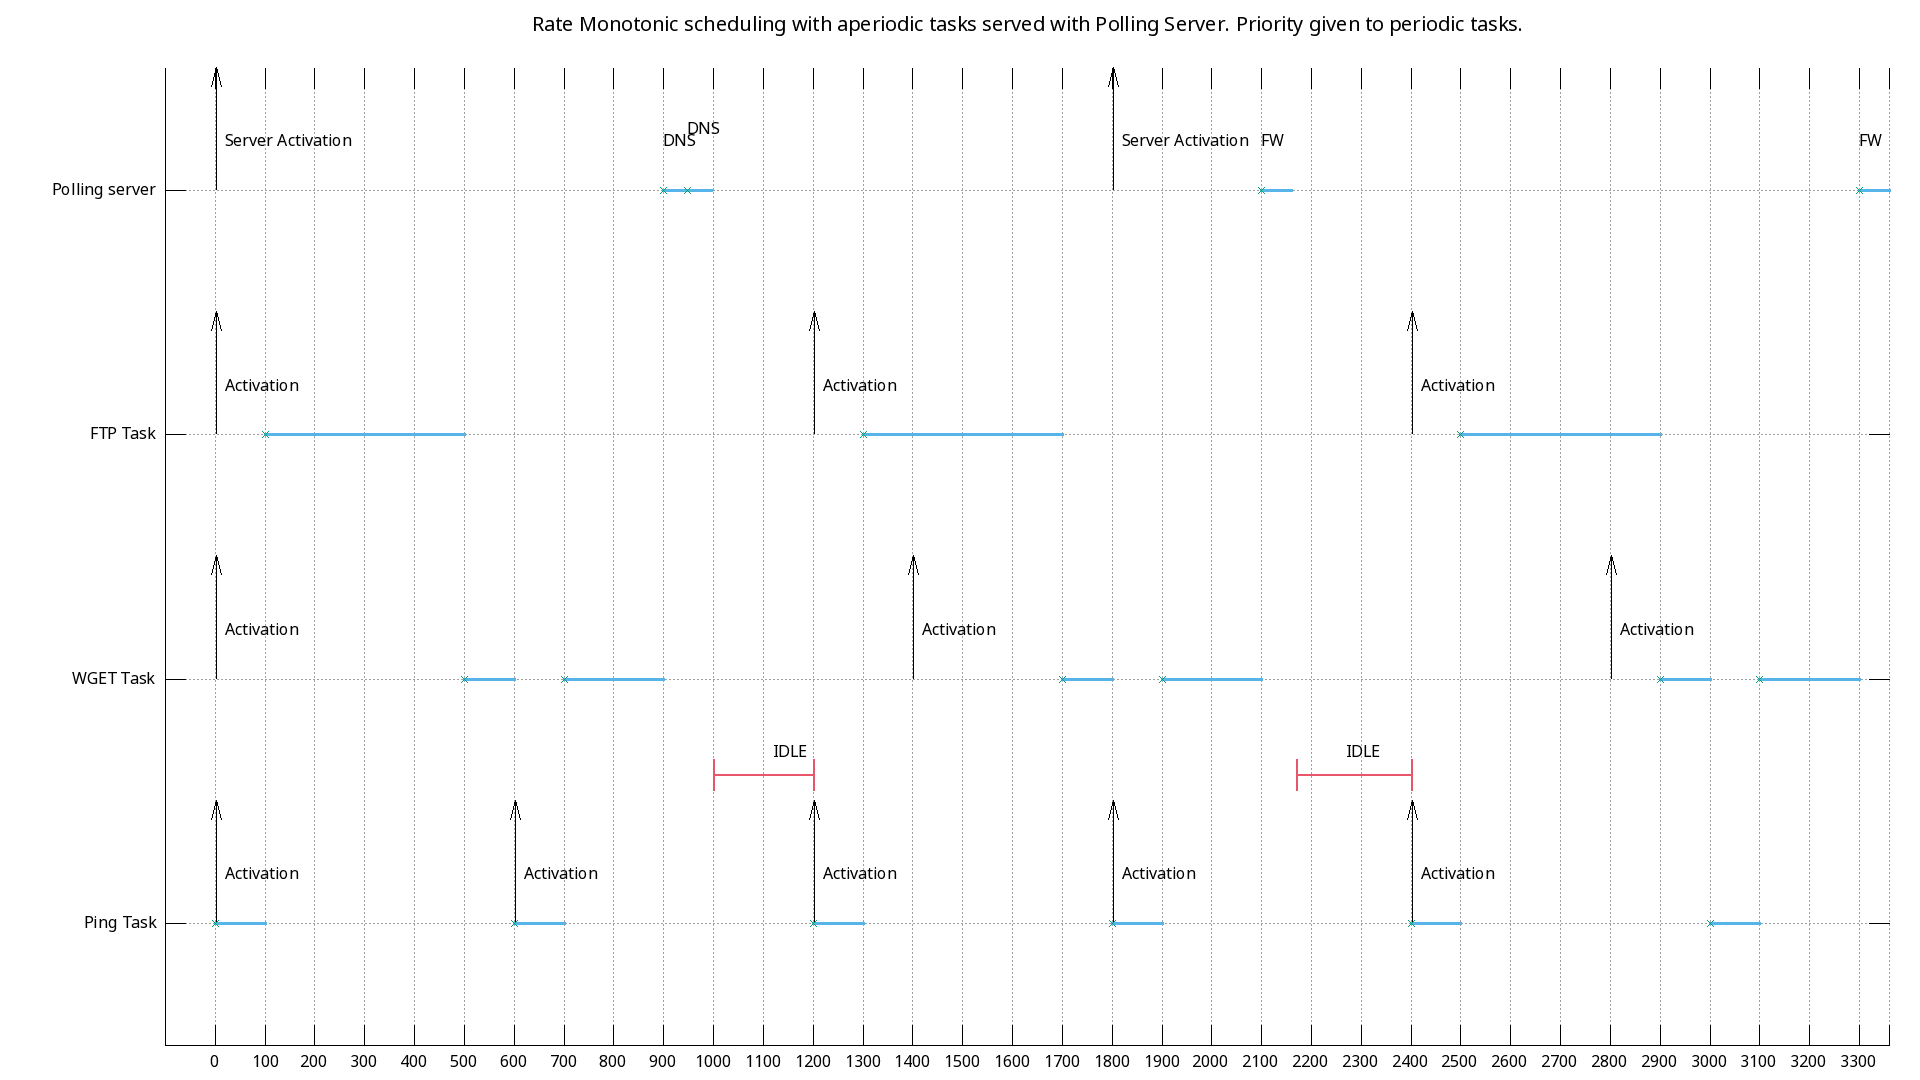
\includegraphics[width=1.0\linewidth]{Pictures/pollings_gantt_1202.png}
    \caption{}
    \label{fig:14}
\end{figure}

The output on screen will resemble this:
\begin{lstlisting}
------------------------------------------------------------------------------
[START] Tick count 1 - Task Client1 - LastWakeTime 0 - Priority 9 
[CLIENT] Client 1 pings: 64 Bytes
[END] Execution time 50 (WCET: 100) - Task Client1
------------------------------------------------------------------------------
[START] Tick count 51 - Task Client3 - LastWakeTime 0 - Priority 8 
[CLIENT] File Transfer Status: 10%
[...]
[CLIENT] File transfer completed!
[END] Execution time 274 (WCET: 400) - Task Client3
------------------------------------------------------------------------------
[START] Tick count 325 - Task Client2 - LastWakeTime 0 - Priority 7 
[CLIENT] Page status: 10%
[...]
[CLIENT] Request completed!
[END] Execution time 181 (WCET: 300) - Task Client2
------------------------------------------------------------------------------
[START] Tick count 506 - Task PS - LastWakeTime 0 - Priority 6 

[SERVER] DNS Update
[PS] Aperiodic Task Server executed - Polling Server Budget = 83

[SERVER] DNS Update
[PS] Aperiodic Task Server executed - Polling Server Budget = 66
[PS] Next Aperiodic Task Server not schedulable - Reset Polling Server Budget to 100

[END] Execution time 34 (WCET: 100) - Task PS
--------*[IDLE]*--------
------------------------------------------------------------------------------
[START] Tick count 600 - Task Client1 - LastWakeTime 600 - Priority 9 
[CLIENT] Client 1 pings: 64 Bytes
[END] Execution time 46 (WCET: 100) - Task Client1
--------*[IDLE]*--------
------------------------------------------------------------------------------
[START] Tick count 1200 - Task Client1 - LastWakeTime 1200 - Priority 9 
[CLIENT] Client 1 pings: 64 Bytes
[END] Execution time 45 (WCET: 100) - Task Client1
------------------------------------------------------------------------------
[START] Tick count 1245 - Task Client3 - LastWakeTime 1200 - Priority 8 
[CLIENT] File Transfer Status: 10%
[...]
[CLIENT] File transfer completed!
[END] Execution time 275 (WCET: 400) - Task Client3
------------------------------------------------------------------------------
[START] Tick count 1519 - Task Client2 - LastWakeTime 1400 - Priority 7 
[CLIENT] Page status: 10%
[...]
[CLIENT] Request completed!
[END] Execution time 185 (WCET: 300) - Task Client2
------------------------------------------------------------------------------
[...]
\end{lstlisting}
\newpage
\section{Adding Feasibility Tests to our algorithms}
We have taken advantage of the extensive literature on scheduling algorithms to write some tests that could help diagnose problems or just understand better what is going on in our system.\\
In general, static scheduling algorithms are suitable for periodic computations with hard deadlines, while dynamic algorithms are better suited for sporadic or aperiodic tasks. The scheduler will always work to determine the optimal sequence for executing computations. A feasible scheduling ensures that the timing constraints of all computations are met. Schedulability analysis hinges upon prior knowledge of the WCET for each computation. \\\\
We know that the \textbf{utilization factor U} represents the fraction of CPU time used by the computation and it is defined by the following equation:
\begin{equation*}
    U_i = \frac{C_i}{T_i}
\end{equation*}
Where $C_i$ is the WCET of the computation $i$ and $T_i$ is the period.
\subsection{Feasibility of RMS}
Let $\Gamma$ = {$\tau_1$,..., $\tau_n$} be a set of n periodic tasks, where each task $\tau_i$ is characterized by a processor utilization $U_i$.\\\\
$\Gamma$ is schedulable with RM if 
\begin{equation*}
    \prod_{i=1}^n (U_i +1) \leq 2
\end{equation*}
If the condition is not valid it does not mean that the algorithm does not work but we can prove that it may still. This feasibility test is also referred as a \textbf{sufficient} but not necessary test under RM schedulability. 

\subsection{Feasibility of EDF}
Schedulability of periodic task set handled by EDF can be verified through the processor utilization factor.\\\\
A set of periodic tasks is schedulable with EDF if and only if:
\begin{equation*}
    \sum_{i=1}^n U_i \leq 1
\end{equation*}
This feasibility test is also referred as a \textbf{sufficient and necessary} test under EDF schedulability.

\subsection{Adding basic feasibility tests inside our code}
The following code is called inside the \verb|vTaskStartRealTimeScheduler| function, to immediately inform the user of the theoretical feasibility of the tasks.
\begin{lstlisting}
static BaseType_t prvCheckFeasibilitySTD( void ){
    #if( we use RMS )
        float xU = 1.0;				// U is CPU Utilization Factor
        float adder = 1.0;			// The constant we need inside the RMS formula
    #elif( we use EDF scheduling )
        float xU = 0.0;
    #endif
    [...]
while( traversing TCB list ){
    
#if( we use RMS )
  xU *= (float) currentTCB->xWCET / currentTCB->xPeriod + adder ; 	// U = U*(WCETi/PERIODi)+1
#elif( we use EDF scheduling )
  xU += (float) currentTCB->xWCET / currentTCB->xPeriod;			// U = U+(WCETi/PERIODi)
#endif
        
        [...]
    }

// test the result against our thresholds:	
	
    #if( we use RMS )
        if( xU > 2 ){
            return false;
        }

    #elif( we use EDF scheduling )
        if( xU > 1 ){
            return false;
        }
    #endif

    return true;
}
\end{lstlisting}
 

\subsection{The Worst-Case Response Time approach}
The utilization factor is just a non-exact test to verify if a set $\Gamma$ of periodic tasks is schedulable with EDF, because if the response is non-negative, it still does not guarantee that all $\tau_i \in \Gamma$ are schedulable.\\\\
As we can see experimentally, this is the case for RMS tests too.
\\All of this has also been demonstrated by numerous studies, using the \textbf{Worst-Case Response Time} (\textbf{WCRT}) analysis approach \cite{10.1093/comjnl/29.5.390}. \\\\
The worst-case response time of a task is the length of the longest interval from a task’s release until its completion. To determine the worst-case response time, we consider the so-called \textit{critical instants}\cite{10.1145/321738.321743}.\\\\
The worst case response time $R_i$ of a task $\tau_i$ is given by the smallest $R$ that satisfies:
\begin{equation*}
\begin{split}
    &R^0 = C_i\\
    &R^{m+i} = C_i + \sum_{j<i} \left\lceil \frac{R^{m}}{T_j} \right\rceil C_j
\end{split}
\end{equation*}
Assuming a critical instant at time zero, the factor $\left\lceil \frac{R^{m}}{T_j} \right\rceil$ gives the worst-case number of preemptions that an execution of task $\tau_i$ suffers from task $\tau_j$ in an interval $[0, n)$ with $( m < n )$. The R is the interval between the release time and the end of the execution of the computation and it defines the WCRT.
The computation is schedulable when the maximum response time
$R_i$ is less than or equal to its deadline ($R_i \leq D_i$). \\
\begin{example}{Note}
This approach is not only suitable for Earliest Deadline First (EDF) scheduling but also provides a necessary condition for Rate-Monotonic (RM) schedulability, where in this scenario the deadline is equal to the period.
\end{example}
\subsubsection{Code implementation}
To implement the WCRT inside our code, we first added a new variable, \verb| TickType_t xWCRT|, to our custom TCB; then, we implemented a new function, \verb|prvCheckFeasibilityWCRT|.\\
In the following excerpt we present \textbf{the iterative procedure we devised to calculate worst-case response times}, calling \textit{I} the $R^{m+i}$ quantity: \\
\begin{lstlisting}
static BaseType_t prvCheckFeasibilityWCRT(void) {

  long int I;
  currentTCB = first TCB of list;

  [...]

  long int R = currentTCB -> xWCET;

  [...]

  if (currentTCB -> WCRT > currentTCB -> Period)
    return FALSE;

  currentTCB = next TCB in list;

  while (traversing TCB list) {
    R = R + currentTCB -> xWCET;

    while (R <= currentTCB -> xDeadline) {
      I = 0;
      [...]
      hpTCB = highest priority TCB in list;
      do {
        [...]
        I = I + (CEIL(R, hpTCB -> xPeriod) * hpTCB -> xWCET);
        hpTCB = next item in list; //get the next highest priority task
      } while (hpTCB != currentTCB);

      I = I + currentTCB -> xWCET;

      if (R == I)
        break;
      else
        R = I;
    }

    if (R > currentTCB -> xDeadline)
      return FALSE;

    currentTCB -> xWCRT = R;
    printf("Task, WCET, WCRT"));

  currentTCB = next TCB in list;
}

return TRUE;
}
\end{lstlisting}

\subsubsection{Pratical example}
Here we present a practical example, using three "Client" Tasks with the following characteristics:
\begin{center}
\begin{tabular}{|c||c|c|c|c|}
\hline 
\rule[-1ex]{0pt}{2.5ex} Task & Period & WCET & WCRT \\ 
\hline 
\rule[-1ex]{0pt}{2.5ex} Ping1 & 300 & 100 & 100\\ 
\hline 
\rule[-1ex]{0pt}{2.5ex} Ping2 & 800 & 300 & 500\\ 
\hline 
\rule[-1ex]{0pt}{2.5ex} Ping3 & 800 & 200 & 800\\ 
\hline 
\end{tabular}
\end{center}

The standard RM feasibility test \textbf{fails}:
\[\bigg{(}\frac{1}{1}+1\bigg{)}\cdot\bigg{(}\frac{3}{8}+1\bigg)\cdot\bigg(\frac{2}{9}+1\bigg)\leq2\] is \textbf{not true}, but we still might be able to get a feasible scheduling with WCRT ... which is exactly what the tests done by our program tell us:

\begin{lstlisting}
U_max > 2

STANDARD FEASIBILITY TEST NOT PASSED

Task Client1 - WCET 100 - WCRT 100
Task Client2 - WCET 300 - WCRT 500
Task Client3 - WCET 200 - WCRT 800

FEASIBILITY WCRT TEST PASSED
\end{lstlisting}

The resulting scheduling is the following:

\begin{figure}[H]
    \centering
    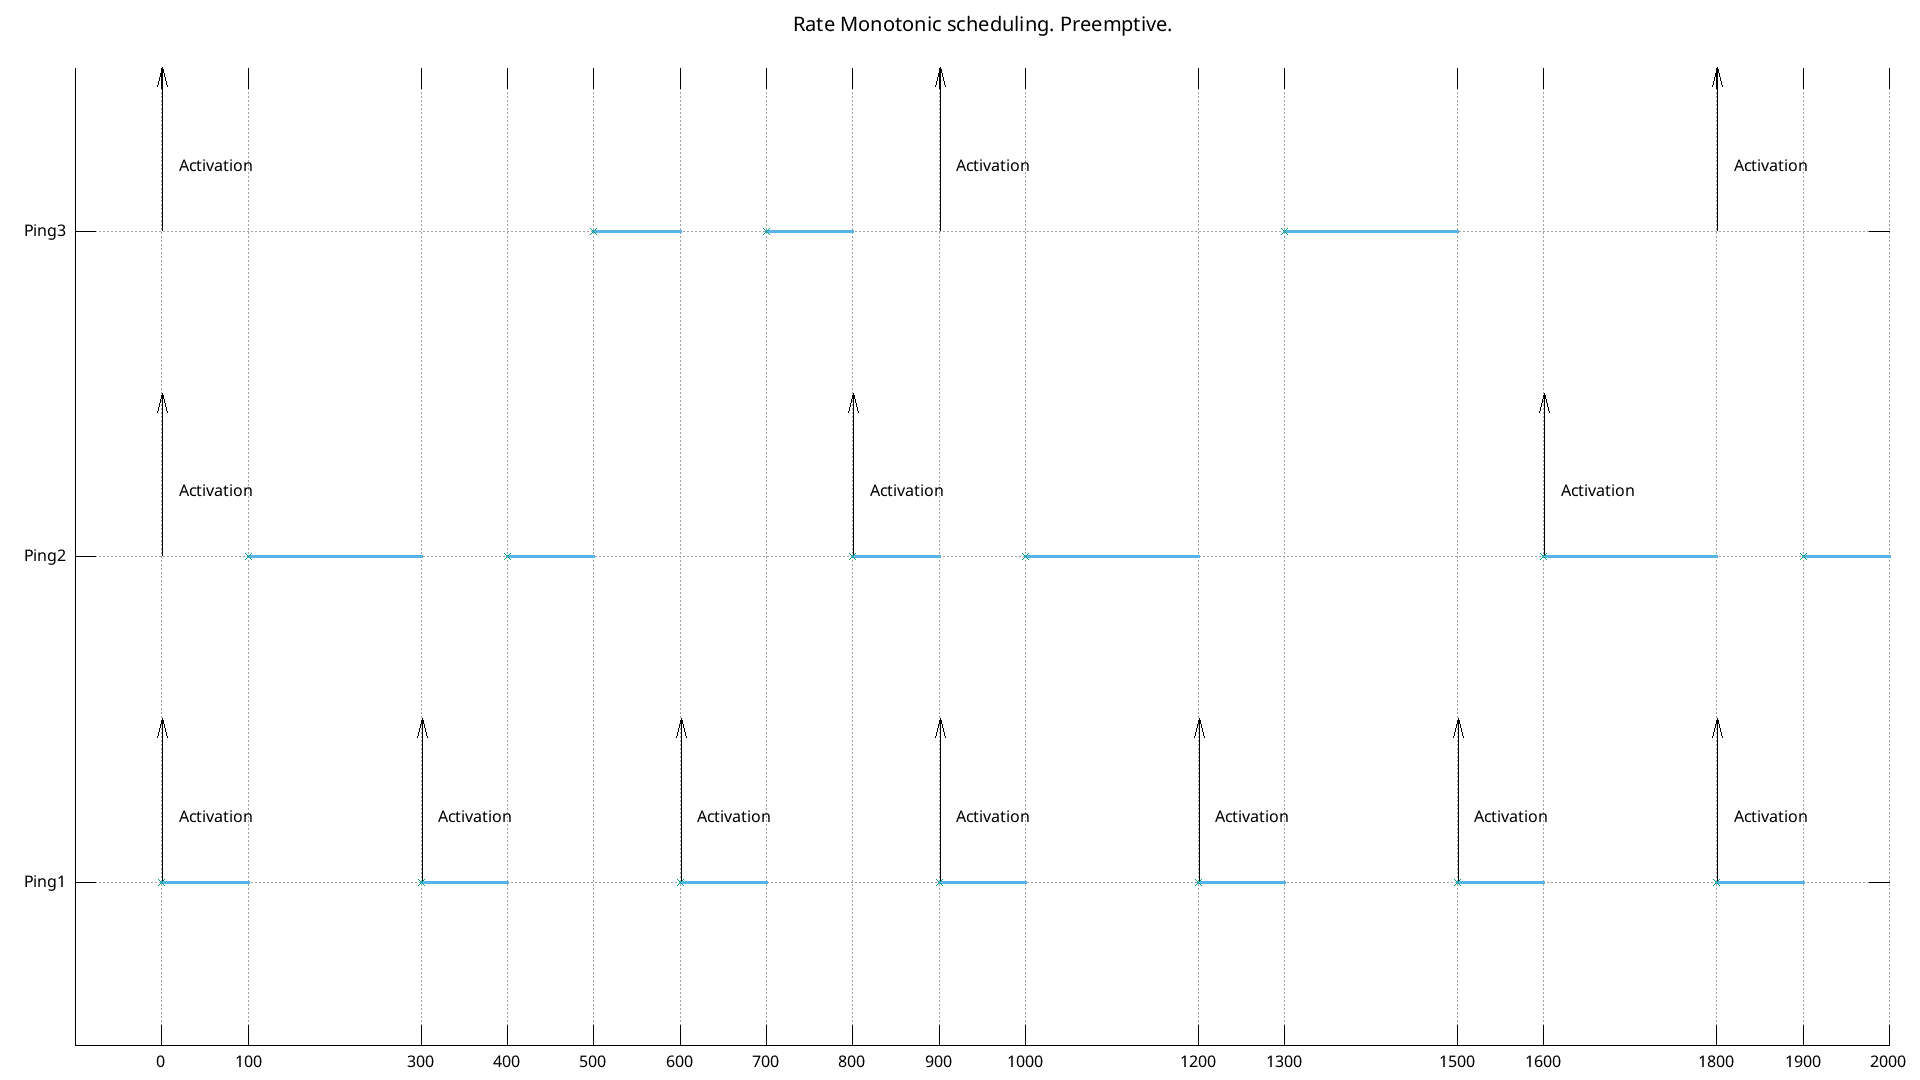
\includegraphics[width=1.0\linewidth]{Pictures/wcrt_gantt_1302.png}
    \caption{}
    \label{fig:13}
\end{figure}

\newpage

%%%%%%% Bibliografia %%%%%%%%
\printbibliography{}
%%%%%%% FINE Bibliografia %%%%%%%%      
\end{document}
